\chapter{Sodium Channels (Na channel)}
\label{chap:Na-channel}

\def\dtsz{{\text{dt}$^\text{sz}$}}

Na+ channel homologs that conduct Ca2+ appeared more than a billion years ago.
Then, sodium-selective $\Na$ channels evolved separately in Cnidaria and
Bilateria (Sect.\ref{sec:cnidarians}) which has structural differences at
channel pore. Ion selectivity is crucial for fast and accurate signaling, and
the emergence of Na+-selectivity likely addressed a need to distinguish neuronal
stimuli from intracellular signaling driven by Ca2+.

We will discuss
\begin{enumerate}
  \item Nav channels - Sect.\ref{sec:Nav-channels}
  
   The ion selective filter is a ring of four amino acids (Asp, Glu, Lys, and
   Ala [DEKA] which is conserved in all vertebrate and many invertebrate Navs.
   The Lys at the third position of the DEKA SF is critical for ion selectivity,
   as indicated by the increase in Ca2+ and K+ conductance when it is
   substituted in mammalian Nav channels.
   
  \item Nav-like channels - Sect.\ref{sec:Nav-like-channels}

   The ion selective filter is a ring of four amino acids (Asp, Glu, Glu, and
   Ala [DEEA] and has been observed in many invertebrates, including arthropods,
   mollusks and tunicates.
     
  \item voltage-independent sodium channel - Sect.\ref{sec:Na-channel-voltage-independent}
\end{enumerate}

\section{Sodium channel vs. Sodium current}

\textcolor{red}{REMEMBER that a particular type of {\bf sodium current} and the
{\bf sodium channel} that underlying that current are two different concepts}.
One sodium current, as estimated from the experiment, can be the result of the
activation of one, two or more types of sodium channels.

The nomenclature of sodium channels was developed in 2000 (Goldin et al.
(2000)). 
\begin{enumerate}
  \item based on {\bf sodium currents}
  
There are mainly two type of $\Na$ current: transient (inactivating) -
Sect.\ref{sec:transient-sodium-current}, and persistent (non-inactivating)
current - Sect.\ref{sec:persistent-sodium-current}. Other types:
resurgent sodium current (Sect.\ref{sec:resurgent-sodium-current}).

Each current can be the result of $\Na$ permeability through one or more types
of $\Na$ channels, e.g. Nav1.6, Nav1.2 (Sect.\ref{sec:Na-channel-structure}).
  
  \item {\bf based on sodium channels}: the subunit isoforms that express the
  transmembrane protein underlying one of the above sodium currents.
\end{enumerate}
% Goldin AL, Barchi RL, Caldwell JH, Hofmann
% F, Howe JR, et al. 2000. Nomenclature
% of voltage-gated sodium channels. Neuron
% 28:365 - 68

\section{Nomenclature}
\label{sec:nomenclature-Na-channel}

We use the parallel nomenclature for ion channel called UCL/HGNC/HUGO Human Gene
Nomenclature symbols which is developped in conjunction with the human genome
project (reference: Sect.\ref{sec:nomenclature-Cav-channels},
Sect.\ref{sec:nomenclature-K_channel}) - review: Trimmer, Rhodes (2004).

Nav channel are primarily in Nav1 family.
Nav channel genes start with {\it SCN}, then a numerical designation followed by
an A for $\alpha$-subunit
\begin{enumerate}
  \item SCN1A = Nav1.1
  \item SCN2A = Nav1.2
\end{enumerate}
EXCEPTION: 
\begin{itemize}
  \item Nav1.6 = SCN8A 
\end{itemize}


\section{Nav channels: Nav1.x}
\label{sec:Nav-channels}
\label{sec:Nav1-family}


Sodium gating currents were first recorded in 1972 by Armstrong and Bezanilla
(1972) at Woods Hole; and shortly after by Rojas and Keynes at Plymouth (1973).
Unlike Nav-like channel (Sect.\ref{sec:Nav-like-channels}), the motif for
selective filter is DEKA in Nav channels (see structure section).

In 1984, Numan and colleagues cloned cDNA encoding of electric eel
electroplax Nav channel $\alpha$ subunit to study the underlying
genes that encode the sodium proteins. This was the first subunit of a
voltage-dependent ion channel to be cloned, lead to the first understanding of
the amino acid  sequence of the gene encoding a voltage-gated ion channel.

Typically, the leak current (I$_g$) and sodium current is recorded; after
subtracting the symmetrical capacitive current
(Sect.\ref{sec:capacitive-current}); and then finally the sodium current is
calculated after subtracting the leak current.

Voltage-independent sodium channels also exist -
Sect.\ref{sec:Na-channel-voltage-independent}.


\subsection{Structure}
\label{sec:Na-channel-structure}

Voltage-gated sodium channels (Nav) are are the founding  members of a
superfamily that include voltage-gated $\K$ channels, voltage-gated $\Ca$
channels, Trp-relatd channels (Sect.\ref{sec:TRP-classification}) and
cyclic-nucleotide-gated channels (Sect.\ref{sec:cyclic-nucleotide}).

In this family
\begin{itemize}
  
  \item $\Na$ channels is the most recent and has evolved from similarly
  structured $\Ca$ channels with a single large pore-forming $\alpha$ subunit;
  and possibly with one or more (regulatory) beta ($\beta$) auxiliary subunit
  (Sect.\ref{sec:Na-channel-beta-subunit}), Fig.\ref{fig:Na-channel-structure}.
  

\begin{enumerate}
  \item alpha subunit (Sect.\ref{sec:Na-channel-alpha-subunit}) control: channel
  opening, ion selectivity, and rapid inactivation
  
  \item beta subunit (Sect.\ref{sec:Na-channel-beta-subunit}) control:
  voltage-dependency of opening and closing
\end{enumerate}

  $\Ca$ channels are probably arose by 2 rounds of gene duplication from
  the ancestors $\K$ and cyclic-nucleotide-gated channels.
  
  \item A single $\alpha$ subunit has 4 homologous repeat
  domains (labeled from I to IV); each domain contains 6 TMs (labeled S1 to S6).
  
  The highly conserved S4 segment (for each domain) acts as the channel's
  voltage sensor (voltage-sensing domain or VSD). VSDs are connected to the pore
  domain through connecting helices S4-5.

%   Whereas the $\alpha$-subunit of Kvs is single pore (one pore) domain -
%   Sect.\ref{sec:K2P}, the $\alpha$-subunits of Cavs and Navs are large monomers
%   of four homologous, nonidentical domains (Hille, 2001).
  
  \item The appearance of 4-domain sodium channels coincided with evolution of
  metazoans that had specialized neurons - Sect.\ref{sec:metazoan-brain}.
  
  From sea anemone {\it Nematostella vectensis}, a member of the early-branching
  metazoan phylum Cnidaria, it revealed a sodium-selective channel bearing a
  noncanonical selective-filter (SF). Phylogenetic study assigns 
  Nematostella Na+-selective channel to a channel group unique to Cnidaria,
  which diverged >540 million years ago from Ca2+-conducting Na+ channel homologs. 
  
\end{itemize}

\begin{figure}[hbt]
  \centerline{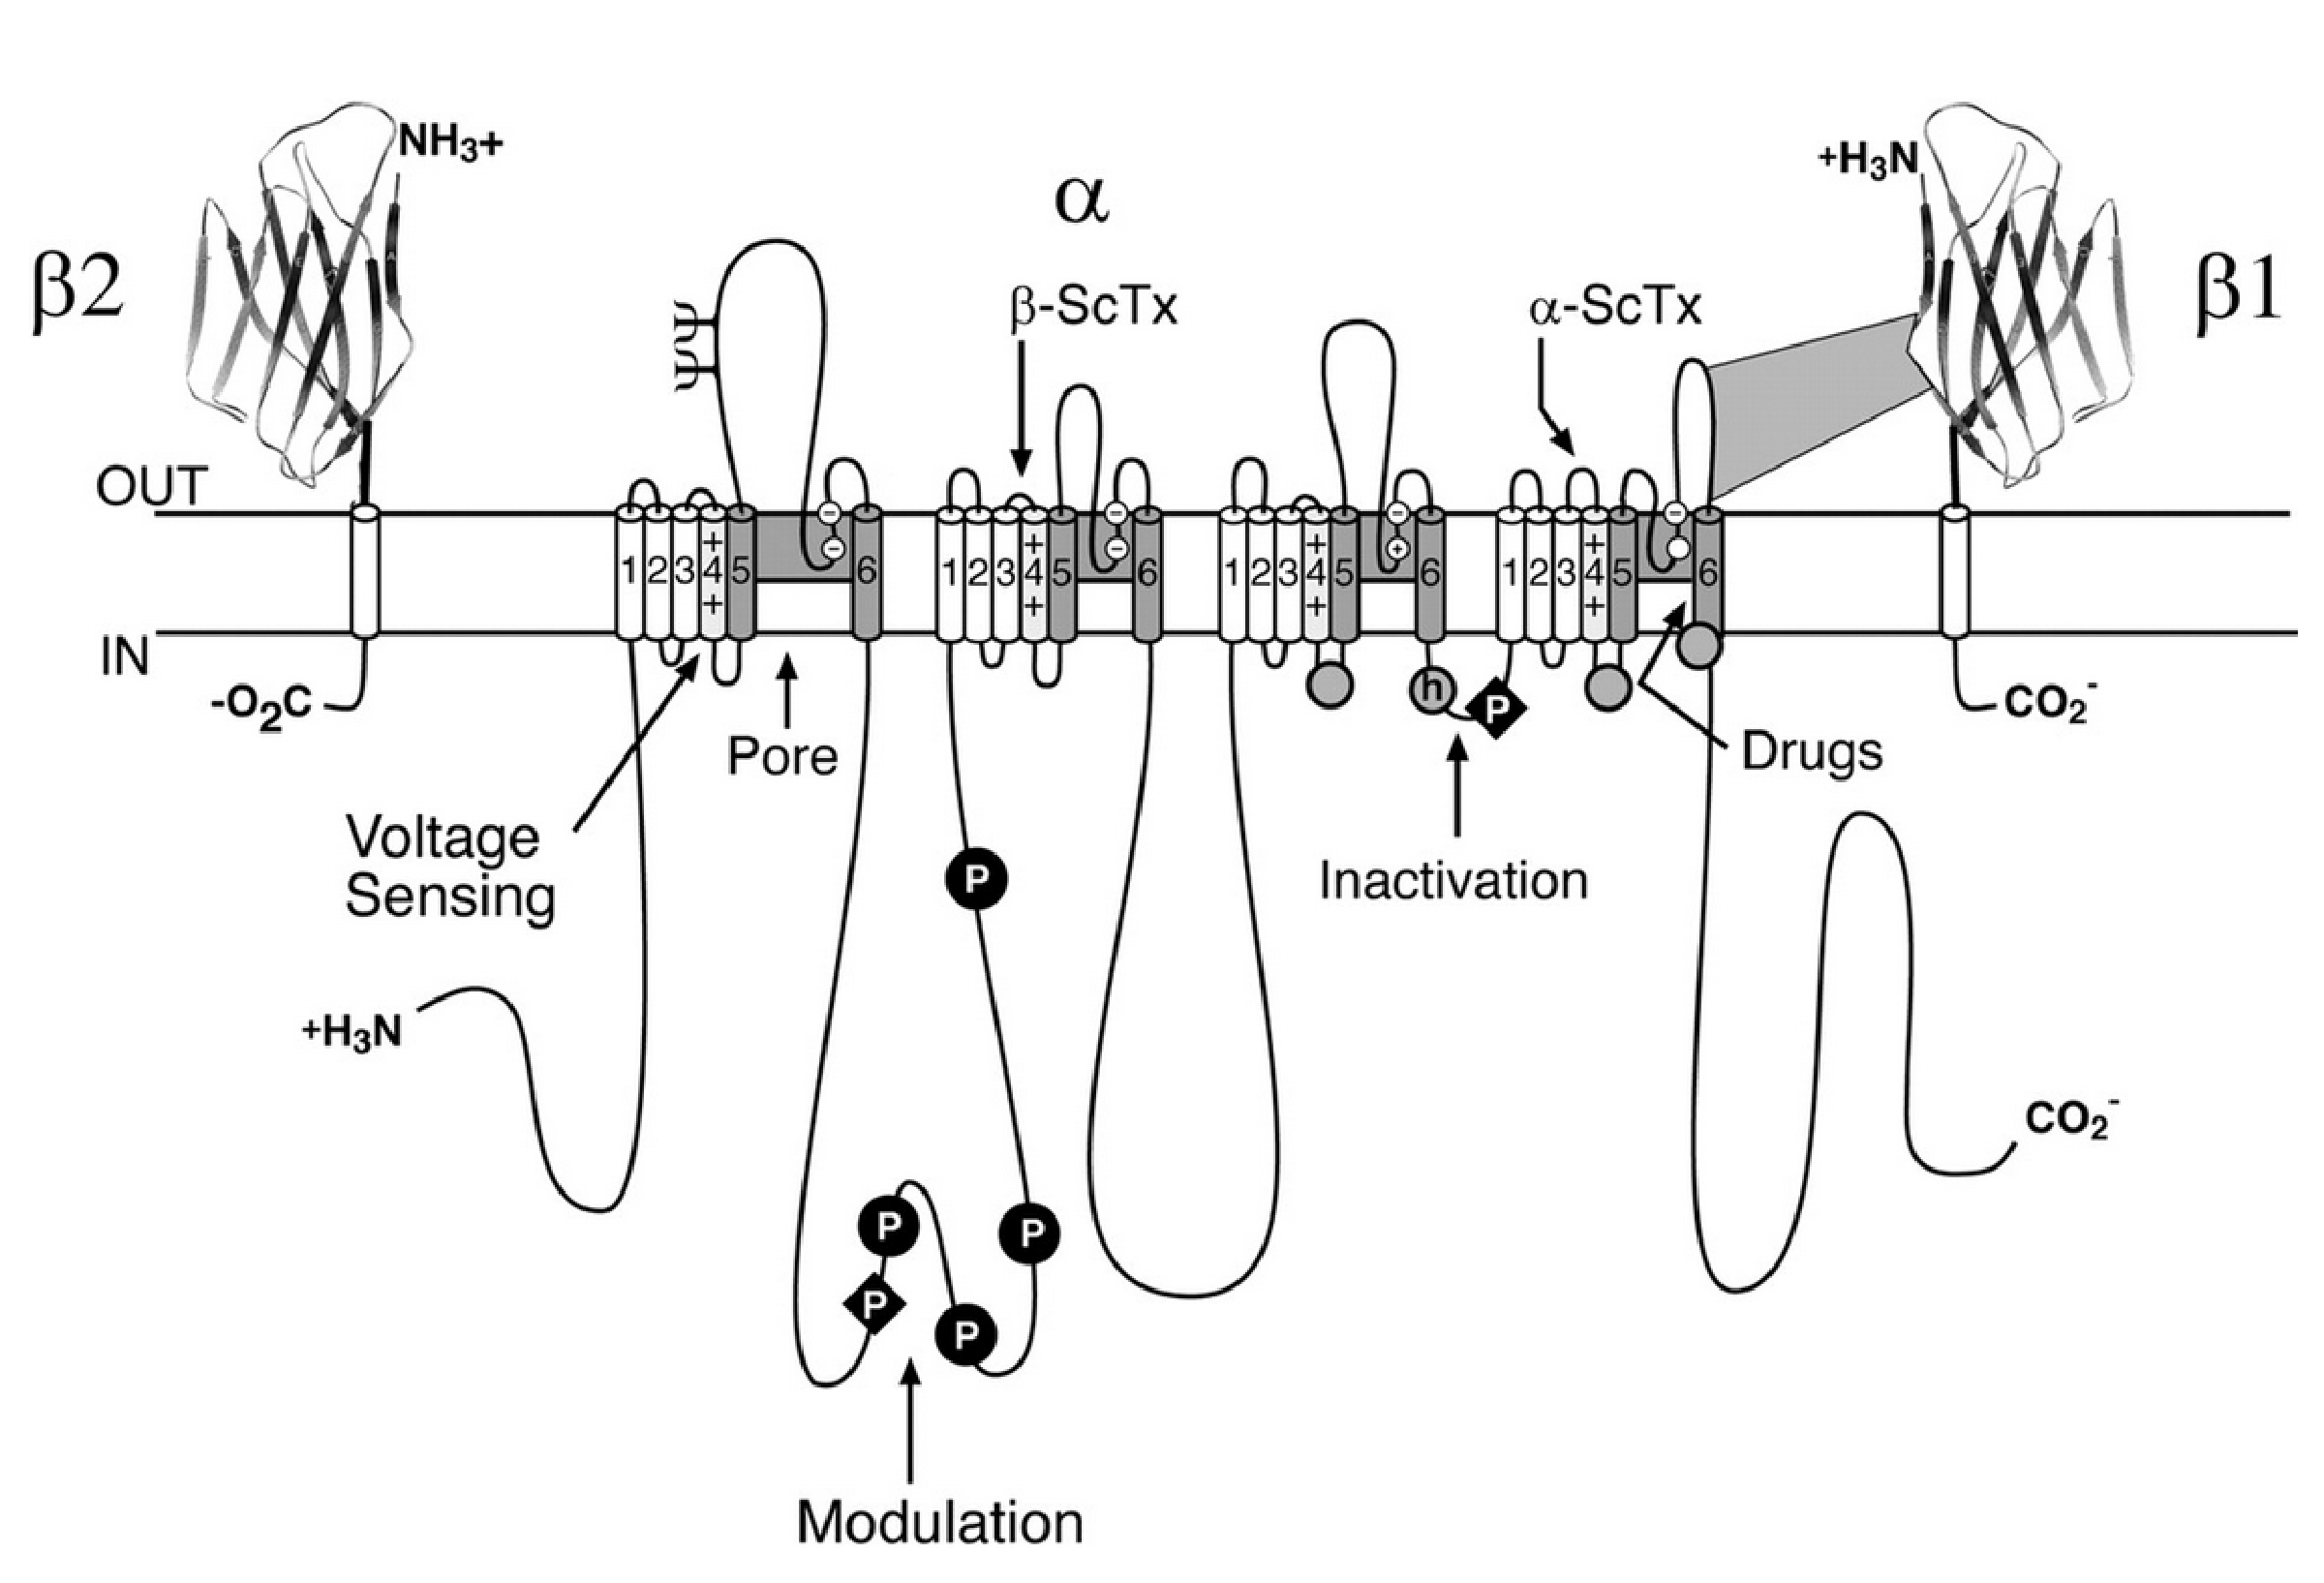
\includegraphics[height=6.5cm,
    angle=0]{./images/Na-channel-structure.eps}}
  \caption{The long ($\approx$ 260kDa) $\alpha$ subunit is organized in four
  homologous domains (I-IV), each of which contain six transmembrane $\alpha$
  helices (S1-S6) and an additional pore loop located between the S5 and S6
  segments.
  The two auxiliary subunits are at extracellular side; $\Psi$: sites of
  probable N-linked glycosylation; P: sites of demonstrated protein
  phosphorylation by protein kinase A (circles) and protein kinase C (diamonds);
  shaded region: pore-lining S5-P-S6 segments; ++: S4 voltage sensors; h in
  shaded circle: inactivation particle in the inactivation gate loop; open
  shaded circles: sites implicated in forming the inactivation gate receptor.
  Sites of binding of $\alpha$- and $\beta$-scorpion toxins (ScTx) and a site of
  interaction between $\alpha$ and $\beta_1$ subunits are also shown}
  \label{fig:Na-channel-structure}
\end{figure}

\subsection{voltage-sensing domain}
\label{sec:voltage-sensing-domain}
\label{sec:VSD-voltage-sensing-domain}

Studies of Kv channels suggested that the voltage-dependent conformational
changes of VSDs, particularly of the gating charge-containing S4 segments, lead
to the opening of the cytoplasmic gate of the pore domain


 \subsection{-- alpha subunit (DEKA selective filter): 9 (Nav1.1-Nav1.9) + 1
(Nax)}
\label{sec:Na-channel-alpha-subunit}
\label{sec:DEKA-motif}



Vertebrate large pore-forming $\alpha$-subunit genes, especially those encoding
the human and rodent sodium channels, are the best characterized to date.  The
$\alpha$ subunit of a sodium channel is of $\approx 260$kDa),
Fig.\ref{fig:Na-channel-structure}.

A single $\alpha$ subunit folds into four homologous domains (I-IV or DI-DIV
(D=domain)), which are similar to one another. Each domain contain six
$\alpha$-helical transmembrane segments (S1-S6), in that S5-S6 segments form the
pore-forming domain. 
 
\begin{itemize}

  \item The voltage sensor is on S4 of each domain, similar to that in $\K$
channel - Sect.\ref{sec:Kv_channel} (Yu, Catterall (2003)).

Upon depolarization, S4 segment moves toward the extracellular side of the
cell membrane, allowing the channel to become permeable to ions

  \item ion-conducting pore: can be broken into 2 regions
  
  \begin{enumerate}
    \item {\it more external (i.e. more extracellular) of the pore}: formed by
    the P-loop between S5 and S6 of each domain.

  A reentrant loop between helices S5 and S6 is embedded into the transmembrane
  region of the channel to form the narrow, ion-selective filter at the
  extracellular end of the pore.
  This portion is the most narrow and in in charge ion selectivity filter (SF) -
  it is a ring of four amino acids (Asp, Glu, Lys, and Ala [DEKA]) that are
  contributed by the pore-lining loops (p-loop) of the four domains
  \citep{catterall2000}.

  The Lys at the third position of the DEKA SF is critical for ion selectivity,
  as indicated by the increase in Ca2+ and K+ conductance when it is substituted
  in mammalian Navs (Heinemann et al., 1992; Schlief et al., 1996).

  Although the DEKA SF is conserved in all vertebrate and many invertebrate Navs
  (Widmark et al., 2011), novel Nav-like channels with a DEEA SF have been
  observed in many invertebrates (Sect.\ref{sec:Nav-like-channels}).
    
  
    \item {\it more internal}: formed by the four repeats that combine S5-S6 of
    each domain.

The four repeats provides structural support for the selectivity filter
(SF) that determines the ion selectivity.

  \end{enumerate}
  
The transmembrane protein with only the pore-forming $\alpha$ subunits are
enough for functional expression, i.e. channel opening, ion selectivity and
rapid inactivation; yet the kinetics and voltage dependence of channel gating
are modified by the presence of auxiliary $\beta$ subunits.
  
  \item {\bf modulating}:
  \begin{enumerate}
    \item The region linking domain I and II: sites of phosphorylation (P): 4
    sites for PKA; and one site for PKC. 
    
    \item The region linking domains III and IV: one site for phosphorylation by
    PKC; and one inactivation site for the channel after prolonged activation.
  \end{enumerate}  
  
\end{itemize}

There are 9 different $\alpha$ subunits: Nav1.1 to Nav1.9. A tenth related
isoform (Na$_x$) may also function as a Na+ channel
(Sect.\ref{sec:Nav1-family-alpha-subunit-based-classification}).
Each $\alpha$ subunit is encoded by at least 20 exons.

\begin{figure}[hbt]
  \centerline{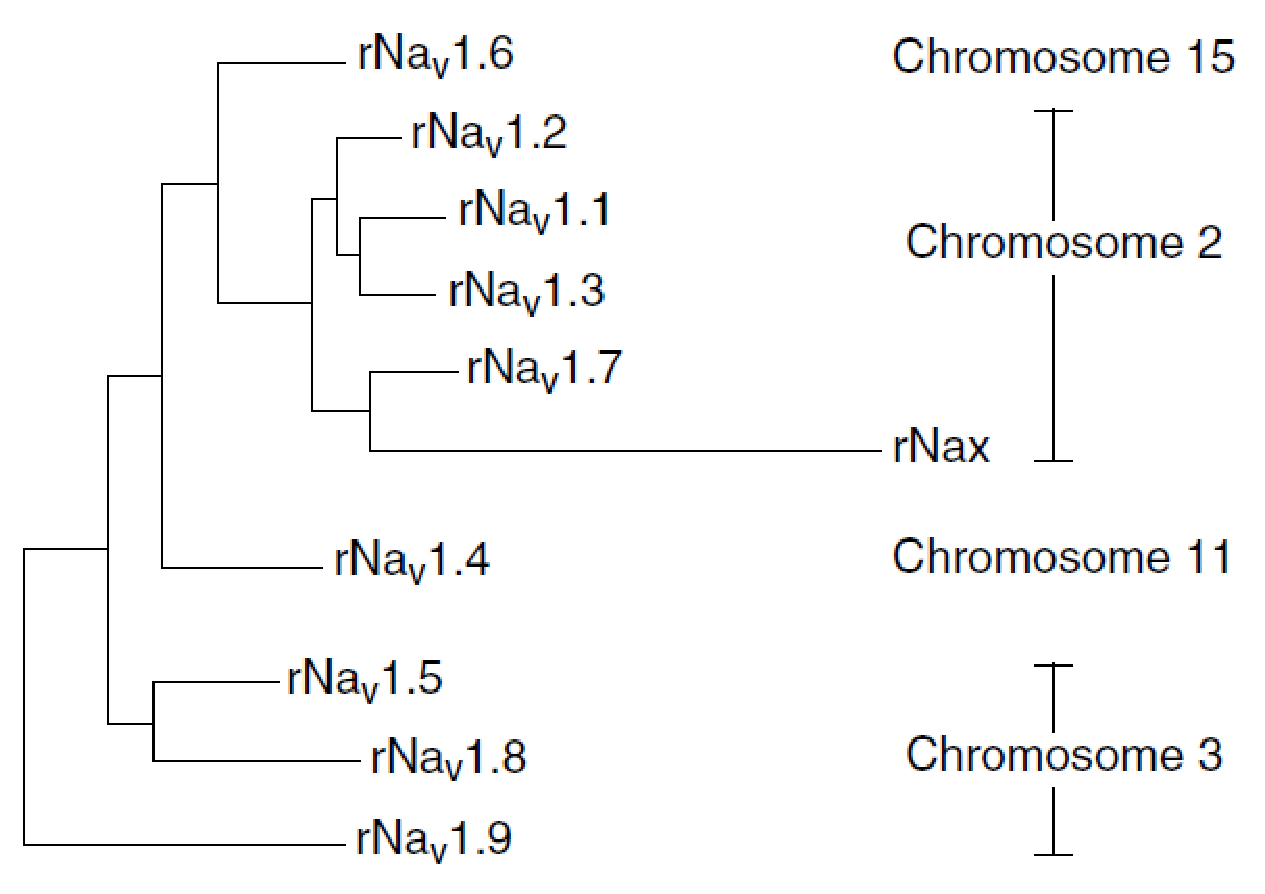
\includegraphics[height=5cm,
    angle=0]{./images/Nav-channel-phylogenetic-tree.eps}}
\caption{Phylogenetic tree of rat Nav channels (rNav) (Yu, Catterall (2003)).
PAUP software (Sect.\ref{sec:PAUP-software-phylogenetic}) is used to construct
the tree; ClustalW is used to analyze protein sequence for grouping. Human
chromosomes with human ortholog gene map to rat Nav is shown on the right side}
\label{fig:Nav-channel-phylogenetic-tree}
\end{figure}

  
\subsection{-- beta subunits: 4 (beta-1 to beta-4)}
\label{sec:Na-channel-beta-subunit}

There are 4 found beta auxiliary subunits in the range 33-36 kDA:
  ($\beta_1$ 36 kDa, $\beta_2$
33 kDa, $\beta_{1A}$ 45 kDa, and $\beta_3$ (not found size), $\beta_4$ (recently
found by (Yu, Catterall (2003))). These subunits are encoded by {\it
Scn1b-Scn4b} genes.

More information about their association to alpha-subunit, read 
\begin{enumerate}
  \item Sect.\ref{sec:Nav-neuronal} for CNS
  
  \item Sect.\ref{sec:Nav-skeletal} and Sect.\ref{sec:Nav-cardiac} for the
  skeletal muscle and the heart, respectively.
  
\end{enumerate}


% 10. Isom LL. (2001) Sodium channel beta subunits: anything but auxiliary.
% Neuroscientist, 7 (1): 42-54. [PMID:11486343] \begin{itemize} \item In CNS:
% 260 kDa $\alpha$ subunit with one or more auxiliary $\beta$ subunit
% ($\beta_1$, $\beta_2$, $\beta_3$) of 33-36 kDa \end{itemize}

\begin{itemize}
  
  \item On the basis of structural and sequence identity, $\beta$
  subunits belong to immunoglobulin superfamily of cell adhesion molecules
  (IgCAMs). The C-terminal of beta-subunit is short and is believed to form an
  immunoglobin domain.

 NOTE: Nav$\beta$1 to Nav$\beta$4, through their extracellular Ig-fold
domains, interact with different $\alpha$ subunits and alter their physiological
properties and subcellular localization.

The residue at Ig-domain interact with ankyrin, tenascin and neurofascin, which
may be responsible for targeting sodium channel complexes to the nodes of
Ranvier.

  \item $\beta_1$ and $\beta_3$ bind covalently to the alpha-subunit via a
  di-sulphide bridge; while $\beta_2$ and $\beta_4$ bind \textcolor{red}{much
  more weakly}.
  
  \item $\beta_1$ and $\beta_2$ subunits function as cell adhesion molecules
  through their extracellular Ig-like domain.

  
  \item $\beta$4 is similar to the $\beta$2 subunit (35\% identity) and contains
  an extracellular Ig-like domain which interacts with $\alpha$ subunits at
  Cysteine  residue.

Overexpression of $\beta$4 induced neurite outgrowth in neuroblastoma cells and
increased spine density in hippocampal cultured neurons, suggesting a
function in cell adhesion as seen for other b-subunits.

This interaction is required for $\beta$4 recruitment at the nodes of Ranvier.
$\beta$4 subunits is thought to underline resurrent sodium current
(Sect.\ref{sec:resurgent-sodium-current}).

It is reported that $\beta$4 is enriched in axon initial segments (AIS) and
nodes of Ranvier of diverse neuronal types in the brain (Buffington et al.
(2013)).

% With similar structure to $\beta_2$, $\beta_4$ is predicted to form an
% extracellular Ig-like fold that might be implicated in such intermolecular
% interaction.

% $\alpha$ subunit has 6 alpha-helical TM segments (S1-S6), with voltage-sensor
% on S4.
 
\end{itemize}



\subsection{-- DEEA selective filter}
\label{sec:DEEA}


A sodium channel with a {\it DEEA} motif (Asp, Glu, Glu, and Ala)  for selective
filter (SF) have been observed in many invertebrates, including arthropods,
mollusks and tunicates (Zhou et al., 2004; Cui et al., 2012; Sato and Matsumoto,
1992; Nagahora et al., 2000)


\subsection{Classification: alpha-subunits}
\label{sec:Nav1-family-alpha-subunit-based-classification}

Ten genes encoding the $\alpha$ (pore-forming) subunit of the voltage-gated
$\Na$ channels (Na$_v$) have been found in different mammalian tissues
\citep{goldin2001}, with similar function
(Sect.\ref{sec:Na-channel-alpha-subunit}). Despite their similarity of function,
the sodium channels were originally named in many different ways, with no
consistent nomenclature for the various isoforms. To eliminate the confusion, a
standardized nomenclature was developed based on $\K$ channels. The number
following the subscript 'v' indicates the gene subfamily (currently only NaV1),
and the number following the full point identifies the specific channel isoform
(e.g., NaV1.1).

There are 9 different mammalian sodium channel isoforms: Nav1.1 to Nav1.9.
\begin{enumerate}
  \item On chromosome 2 (human + mouse): Nav1.1, Nav1.2, Nav1.3, and Nav1.7
  
  These channels are TTX-sensitive and is blocked by TTX at nanoMolar
  concentration
  
  \item On chromosome 3p21-24: Nav1.5, Nav1.8 and Nav1.9

  They have amino-acid sequence that modify TTX-sensitivity wit varying degree
  of TTX resistance (Sect.\ref{sec:TTX-resistant-Nav1-group-2}). 
  
\end{enumerate}

Besides the 9 different isoforms, there are also a closely related sodium
channel-like proteins have been cloned from mouse, rat, and human but have not
yet been functionally expressed (Nax).
These Nax channels are approximately 50\% identical to the NaV1 subfamily of
channels but more than 80\% identical to each other
(Sect.\ref{sec:Nax-channels}).


Lab: \url{http://www.hg.med.umich.edu/labs/meislerlab/research.php}

\subsection{-- group 1 (TTX-sensitive): Nav1.1, Nav1.2, Nav1.3, and Nav1.7}
\label{sec:TTX-sensitive-Nav1}

There are different groups of TTX-sensitive Nav channels. Here we discuss group
1. Other groups: 3 (Sect.\ref{sec:TTX-sensitive-Nav1-group-3}) and 4
(Sect.\ref{sec:TTX-sensitive-Nav1-group-4}). The level of TTX required for
blocking is given in Sect.\ref{sec:Nav-blockers}.

\textcolor{red}{Nav1.1, Nav1.2, Nav1.3, and Nav1.7 are located on chromosome 2}
in both human and mouse (chromosome 2q24); and thus they are the most closely
related group based on phylogenetic tree analysis. They are TTX-sensitive
(Sect.\ref{sec:Na-current-TTX-sensitive}).
   
\begin{itemize}
  
    \item Nav1.1 (former name: rat I (for rat), HBSCI (for human), GPBI (for
    guinea-pig), SCN1A): encoded by SCN1A gene (sodium-channel,
    voltage-gated, type I alpha subunit found in chromosome 2q24.3) -
    Sect.\ref{sec:Nav1.1}
   
  \item Nav1.2: encoded by SCN2A (found in chromosome 2q24.3)
  
  \item Nav1.3: encoded by SCN3A (found in chromosome 2q24)

  \item Nav1.7: encoded by SCN9A
\end{itemize}  


\subsection{-- group 2 (TTX-resistant): Nav1.5, Nav1.8 and Nav1.9}
\label{sec:TTX-resistant-Nav1-group-2}


Nav1.5, Nav1.8, and Nav1.9 are on chromosome 3p21-24; and thus they are also
closely related with amino acid sequences of $> 64\%$ identical.
They are TTX-resistant (Sect.\ref{sec:Na-current-TTX-resistant}) to
varying degrees due to changes in amino acid sequence at a single position in
domain I.

\begin{itemize}
    \item Nav1.5 (LQT3): the principal cardiac isoform, encoded by SCN5A (found in
  chromosome 3p21) \citep{marban1998} - Sect.\ref{sec:Nav1.5-cardiac}.
   
   In the cardiac isoform Nav1.5 (Sect.\ref{sec:Nav1.5}), a
  single amino-acid change from Phenylalanin to Cysteine in the pore-region of
  domain I is responsible for 200-fofld reduction in TTX-sensitivity (relative
  to channels encoded by genes on chromosome 2).
  
   \item Nav1.8 and Nav1.9: these two channels are preferentially expressed in
   peripheral sensory neurons.
   
   The amino-acid residue change from Serine to Cysteine result in even greater
   resistance to TTX 
    
\end{itemize}  

\subsection{-- group 3: Nav1.4 (TTX-sensitive) in skeletal}
\label{sec:TTX-sensitive-Nav1-group-3}

There are different groups of TTX-sensitive Nav channels. Here we discuss group
3. Other two groups: 1 and 4. 

Nav1.4 is tetrodotoxin sensitive (non selective).
Nav1.4: encoded by SCN4A (found in chromosome 17q23.3 of human; chromosome 11 of
mouse and chromosome 10 of rat).

Nav1.4 is expressed at high levels in adult skeletal muscle, at low levels in
neonatal skeletal muscle, and not at all in brain or heart. Nav1.4 channels are
located in the sarcolemma and T-tubular membranes, with a high density near the
endplate of the muscle cell.

Mutations in this gene have been linked to several myotonia and periodic
paralysis disorders
\begin{itemize} 
  \item Mutations in NaV1.4 channels increase channel activity by impairing fast and/or
slow inactivation causing hereditary sodium channelopathies of skeletal muscle,
e.g. muscle stiffness.
  
\end{itemize}

CaM (Calmodulin) regulates the current density of NaV1.4. Association with CaM
is important for functional expression of NaV1.4. Disrupting the interaction
between CaM and the C terminus of NaV1.4 reduced current amplitude by 99\%.

\url{http://channelpedia.epfl.ch/ionchannels/123}

\subsection{-- group 4: Nav1.6 (TTX-sensitive nanoMolar range)}
\label{sec:TTX-sensitive-Nav1-group-4}

Nav1.6: encoded by SCN8A (found in chromosome 12q13.1 in human; chromosome 15
in mouse; and chromosome 7 in rat).

Nav1.6 is highly abundance in the CNS (Sect.\ref{chap:CNS}), with greater than
85\% sequence identity and similar functional properties to channels encoded by
genes on chromosome 2 (Sect.\ref{sec:TTX-sensitive-Nav1}), i.e. TTX-sensitive
in nanoMolar range. However, phylogenetic analysis show a more distant
evolutionary relationship to channels on chromosome 2,
Fig.\ref{fig:Nav-channel-phylogenetic-tree}.

No evidence was found that CaM modulates the voltage dependence of activation or
inactivation of either Nav1.4 or Nav1.6 channels.  Calmodulin also was able to
modulate the inactivation kinetics of Nav1.6, but not Nav1.4, currents in a
calcium-dependent manner.
Disrupting the interaction between CaM and the C terminus of of Nav1.6 reduces
the current amplitude by 62\% (Herzog - Cummins, 2003).




\section{NaChBAC (Nav1 in bacteria): NavRh}

NaChBac is a bacterial voltage-gated sodium (Nav) channel that shows sequence
similarity to voltage-gated calcium channels [Zhang et al, 2013]. 
\url{https://www.ncbi.nlm.nih.gov/pmc/articles/PMC3587708/}
\begin{itemize}
  \item  NavRh, a marine bacterial NaChBac ortholog: two $\Na$ binding sites
  
  The extracellular Na+ ion first approaches site 1 constituted by the side
  groups of Ser181 and Glu183, and then spontaneously arrives at the
  energetically more favorable site 2 formed by the carbonyl oxygens of Leu179
  and Thr178. Na+ permeates through the selective filter in an asymmetrical
  manner, a feature that resembles that of the mammalian Nav orthologs, i.e.
  more inward than outward.
  
  Compared to $\Ca$ channels: Ca2+ ions are prone to being trapped by Glu183 at
  site 1, which then blocks the entrance of both Na+ and Ca2+ to the vestibule
  of the selective filter (SF).
  
  
 
\end{itemize}


\subsection{NavRh}

NavRh has two Na+ binding sites are identified in the selectivity filter (SF) in
Zhang et al. (2013) simulation.
\url{https://www.ncbi.nlm.nih.gov/pmc/articles/PMC3587708/}



\section{Nav-like channels: Nav2.x}
\label{sec:Nav-like-channels}    
\label{sec:Nav2-family}    

The type 2 channels (Nav2.x) are approximately 50\% identical to the type 1
channels (Sect.\ref{sec:Nav1-family}), with significant differences in
regions that are critical for channel function.

Nav-like channels emerged before nervous systems or multicellularity evolved.
Novel Nav-like channels with a {\it DEEA} motif (Asp, Glu, Glu, and Ala)  for
selective filter (SF) have been observed in many invertebrates, including
arthropods, mollusks and tunicates (Zhou et al., 2004; Cui et al., 2012; Sato
and Matsumoto, 1992; Nagahora et al., 2000). NOTE: The Nav channels have DEKA
motif as selective filter (Sect.\ref{sec:Nav-channels}).

Channels with DEKA SF are termed Nav1 (Sect.\ref{sec:DEKA-motif}); while those
with DEEA SF are coined Nav2 (Sect.\ref{sec:DEEA}).
There are five Nematostella channels as NvNav2.1 - 2.5 (Barzilai et al., 2012).
%https://www.ncbi.nlm.nih.gov/pmc/articles/PMC3809514/
\begin{itemize}
  
  \item  exhibited slowly developing activating and inactivating currents in
  response to depolarizing voltage pulses, and substantial tail currents when
  returned to a holding potential
  
  
  
\end{itemize}

Still, only two of these Nav-like channels, BSC1 of the cockroach Blattella
germanica and DSC1 of Drosophila melanogaster, have been functionally expressed
and shown to preferably conduct Ca2+ (Zhang et al., 2011; Zhou et al., 2004).

\section{Nax channels}
\label{sec:Nax-channels}

Nax channels have been cloned from mouse, rat, and human but have not yet been
functionally expressed (Nax). These Nax channels are approximately 50\%
identical to the NaV1 subfamily of channels (Sect.\ref{sec:Nav-channels}) but
more than 80\% identical to each other.

It is suggested that the Nax may not function as a voltage-dependent sodium
channels; but at as a salt sensor. Indeed, Nax KO mice have deficits in sensing
extracellular salt levels in hypothalamus. 

\section{Voltage-independent sodium channel}
\label{sec:Na-channel-voltage-independent}

Sodium channels that are not voltage-gated also exist in biology
though they are structurally unrelated to voltage-gated sodium channels.

Example: the epithelial sodium channels (EnaC) of the EnaC/degenerin (DEG) gene
family mediate sodium transport in epithelia.

We won't focus on this channel further.

\chapter{Nav 1.x channels}
\label{chap:Nav-channels}

The overview of Nav1.x channels is given in Sect.\ref{sec:Nav1-family}.
In this chapter, we will go into details.


\section{Distribution of Nav channels}
\label{sec:Nav-detection-techniques}

Two brain isoforms, Nav1.1 and Nav1.6, have very distinct cellular and
subcellular expression. 

Different techniques to identify Na+ channels
\begin{enumerate}

  \item Using eel Nav channel cDNA, Numa and colleagues were later able to
isolate and identify sequence 3 different rat brain Nav channel
alpha-subunits: Nav1.1 (SCN1A), Nav1.2 (SCN2A), and Nav1.3 (SCN3A).

Nav1.1 mRNA was found highly expressed in {\bf cerebellum}; and at lower levels
in striatum, hippocampus, and thalamus; while it is undetectable in cortex.
  
  \item Autoradiographic localization of specific bound, e.g. I-labeled scorpion
  toxin (but not useful as a label for Na+ channel in intact neural tissue or
  slices)
  
  Detected high level of Na+ channel in AIS of cultured spinal cord neurons, and
  in neurites compared to the cell bodies (i.e. soma) of cultured brain neurons
  
  
  \item Immunocytochemical methods (e.g. using polyclonal antisera) against Na+
  channel purified from rat brain
  
  NOTE: polyclonal antisera reacts poorly with Na+ channels from peripheral
  nerve or skeletal muscle; i.e. more specific to Na+ channels from CNS.
  [Wollner, Catterall, 1986]
  
  NOTE: The technique does NOT allow quantitative estimates of channel density.
  
  \item Ankyrin-G (a membrane protein) is $\Na$ channel-associated protein which
  can be used to identify the region at which $\Na$ channel expressed
  (Purkinje cells in mouse cerebellum) [Zhou et al., 1998]
  
  Na+ channels colocalized with isoforms of the membrane-skeletal protein
  ankyrin-G at axon initial segments, nodes of Ranvier, and postsynaptic folds
  of the mammalian neuromuscular junction.
  This isoform at AIS and node of Ranvier, is 480- and 270-kD alternatively
  spliced variants of ankyrin-G, respectively.
  
   \item Antibody:
   
   Nav1.2(green)
   
   Pan-alpha antibody : recognize both Nav1.2 and Nav1.6
   
    
\end{enumerate}


% In cardiac, the $\Na$ current is generated mainly by the cardiac isoform
% (Na$_v$1.5). 
\begin{enumerate}
  \item  group 1 (NaV1.1, NaV1.2, NaV1.3, and NaV1.7) are broadly expressed in
  neurones; yet with different subcellular distribution.

Nav1.1 mRNA was found highly expressed in {\bf cerebellum}; and at lower levels
in striatum, hippocampus, and thalamus; while it is undetectable in cortex.

Nav1.1. polypeptide was found predominantly in cell bodies and dendrites of
expressing cells. 
Nav1.1. polypeptide was found predominantly in cell bodies (somas) and dendrites
of expressing cells. Nav1.1 is found predominantly in soma and proximal AIS of
fast-spiking GABAergic neurons. (Maurice, Surmeier, 2004) found Nav1.1 mRNA in
all cholinergic interneurons.


Nav1.2 mRNA has a similar pattern of cellular expression like Nav1.1; while
Nav1.2 polypeptide was found specifically localized to axons and terminals,
especially Nav1.2 is the predominant at nodes of Ranvier during early
stage of developmental myelination. So, in the non-myelinated portions, Nav1.2
is highly expressed (in the absence of nav1.6).

(In rodents) Nav1.3 was found at highest level mainly at early stage of
delopment, i.e. embryonic and early postnatal brain. 

In human brain, Nav1.3 has a somatodendritic localization, similar to that
observed in Nav1.1.
  
  \item group 2 (Nav1.5, Nav1.8 and Nav1.9) are highly expressed in heart and
  dorsal root ganglion neurons. 

  Nav1.5 is transiently expressed in developing skeletal muscle but is replaced
  by Nav1.4 in the adult.
  
  Interestingly, Nav1.5 has recently been reported to be expressed at both mRNA
  and protein level in mammalian brians. In mouse brain, Nav1.5 is localized to
  axons.
  
  Nav1.5 is not founed in cholinergic interneurons (Maurice, Surmeier, 2004).
  
  Nav1.8, Nav1.9: preferentially expressed in peripheral sensory neurons.


  \item NaV1.4, expressed primarily in skeletal muscle, and 
  
  \item NaV1.6, expressed primarily in the central nervous system (CNS) with
  high abundant.

Nav1.6 mRNA is highly expressed in cerebellar granule cells, and in (pyramidal
and granule cells) of hyppocampus. 

In many central neurons, Nav1.6 is found as the soma and dendrites of such
cells. Interestingly, Nav1.6 is also found as the principal Nat current at
distal axon initial segment (AIS), nodes of Ranvier of both fast-spiking
GABAergic and excitatory neurons. Nav1.6 is found at high level in conjunction
with Nav1.2 in some cells. Nav$\beta$4 is also enriched in AIS of fast-spiking
GABAergic neurons (Sect.\ref{sec:resurgent-sodium-current}).

At early state of developmental myelination, i.e. nodes of Ranvier initially
formed, Nav1.2 channel is the dominant (while Nav1.6 is not present); and then
with further maturation of the node, Nav1.6 becomes the predomiant. Thus, in
adult neurons with myelinated axons, Nav1.6 expressed at high densities at nodes
of Ranvier.

(Maurice, Surmeier, 2004) found Nav1.6 mRNA in large subset of cholinergic
interneurons; while Nav1.2 mRNA is only detected in one-half of the samples.

% Nav1.6: highly abundant in CNS
  
\end{enumerate}

NOTE: Nav1.1, Nav1.2, Nav1.3, Nav1.4 and Nav1.6, are called neuronal isoform
of Na channels as they are found in the CNS and adult skeletal muscle.


\begin{itemize}
  \item Nav1.1:
  
Early studies showed hippocampal  pyramidal cells  and  dentate  gyrus granule
cells  express  Nav1.1  in  their somata and dendrites. Later studies showed an
opposite result.
% localized to somata and dendrites of neurons (Westenbroek et al., 1989; Gong
% et al., 1999).
   \begin{enumerate}
     
     \item in developing neocortex: Nav1.1 .is predominantly found in AIS of
     parvalbumin-positive (PV) interneurons
     (Sect.\ref{sec:parvalbumin-positive-interneuron}), and in axons and somata
     of a subpopulation of layer V pyramidal excitatory neurons

Here, Nav1.1 is involved in sustained high-frequency firing of neocortical
fast-spiking interneuron (Ogiwara et al., 2007).

     \item in hippocampus: predominantly distributed within somata and axons of
     PV interneurons.

NOTE:  pyramidal neurons express Nav1.1 at extremely low levels
   \end{enumerate}

%  \item 
\end{itemize}

NOTE: The proteins encoded by these genes are also found in the heart, though
with a much lesser expression level (detected using mRNA level), representing
between 5\% to 30\% of total $I_\na$ \citep{brette2006}.


In skeletal:
\begin{enumerate}
  \item \citep{brette2006} (rat): Na channel density is about 4-times higher at the cell
    surface than at the T-tubule \citep{jaimovich1976}
\end{enumerate}
  
%     Na$_v$1.1, Na$_v$1.2,
% Na$_v$1.3, Na$_v$1.4, and Na$_v$1.6
  

\section{Nav channel's kinetics}
\label{sec:i_na-channels}
\label{sec:Nav-channel-kinetics}

Even though Nav channels can be studied in isolation in cell lines or in
oocytes; the lacking of associated subunits, e.g. $\beta$ subunits, make it hard
to know whether the characteristics recorded in these expression systems
accurately reflect the in vivo properties of the channels.

\begin{equation}
I_\na = g_\na (V_m-E_\na)
\end{equation}
with $g_\na$ is the conductance (a measure of permeability of the membrane to
$\Na$ ions).  The probability that a sodium channel is open increase steeply wih
membrane potential in the range near -50mV.

The $I_\na$ current normally open briefly ($\approx 1$ms) and then quickly
inactivate, producing a large inward current that rapidly extinguishes. Once
inactivated, the channels normally cannot reopen until the membrane
hyperpolarizes (during diastole).

To estimate the channel density (N, number of channels), the maximum conductance
($\bar{G}$, mS/pF) was divided by the conductance of a single channel ($\gamma$,
i.e. $\bar{G}=\gamma N$ \citep{hille1978ice}).





\subsection{Drug target}

The fast sodium channels ($I_\na$) are important in generation
the AP, and serve as the primary site for antiarrhythmic drug action. As the
matter of fact, $\Na$ channel is the target of many drug in heart disease
treatment (see Sect.\ref{chap:cardiac-diseases}).
Class I antiarrhythmias drugs are those targeting $\Na$ channels, e.g.
lidocaine, quinidine. To increase the flow of ions along the electrochemical
gradient, we can use {\bf ionophores}, compounds that enter membranes to act as
pathways for ions.


All of the pharmacological agents that act on sodium channels have receptor
sites on the $\alpha$ subunits. At least six distinct receptor sites for
neurotoxins and one receptor site for local anesthetics and related drugs have
been identified
\begin{enumerate}
  \item neurotoxin binding site 1
  \item ..
  \item neurotoxin binding site 6:
  \item local anesthetics binding site:
\end{enumerate}
\url{http://www.guidetopharmacology.org/GRAC/FamilyIntroductionForward?familyId=82}

\subsection{$[\Na]_i$ concentration}

The extracellular $[\Na]_o = 156$mM. There is less change in $[\Na]_i$ during
ECC cycle. However, under different different stimulus frequency and/or HF
condition, the level of $[\Na]_i$ can change significantly. The intracellular
$[\Na]_i$ depends on the ionic strengths, pH and the composition of the
solutions used during the isolation of the cardiac myocytes.
The typical resting range is 5-13 mM.

Sodium-binding benzofuran isophthalate (SBFI) is the most widely used
$\Na$-sensitive fluorescent indicator \citep{minta1989Na}.
\citep{Grupp1985} used Sprague-Dawley rats (175-200mg, body temperature) gave
quiescent $[\Na]_i = 8.5\pm 2.6$ mM and $V_\rest=-79.2\pm 2.4$ mV.
\citep{Shattock1989} estimated resting $[\Na]_i=12.7\pm 0.6$ mM (rat) and
$7.2\pm 0.5$ mM (rabbit).
\citep{Levi1994} estimated quiescent $[\Na]_i=10.9\pm 0.74$ mM in rat (which
gives reversal potential of NCX is -35mV), and significantly lower in rabbit:
$[\Na]_i=3.8\pm 0.23$mM (which give reversal potential of NCX is +45mV).

\citep{Baartscheer2003} (rabbit) investigated the change in $[\Na]_i$ under
control and HF condition at different stimulation frequency (0.2-3Hz), giving
\begin{enumerate}
  \item Control (rabbit): $[\Na]_i$ from 3.8 mM to 6.4mM
  \item HF: $[\Na]_i$ from 6.4 to 10.8 mM
\end{enumerate}

\citep{Baartscheer1997} (rat) estimated control $[\Na]_i=9.6 \pm 0.4$ mM using
SBFI in emission ratio mode. The method is consider better as it doesn't need
micro-electrodes which disrupt the cell membranes. In addition, they
suggested using the fluorescent probe in dual emission mode, rather than
dual excitation mode. The high end of the range, i.e. 20 mM, is unlikely as it
would implicate reversed mode operation of NCX.


Using 1- to 3-day neonatal rat cardiomyotes, \citep{Katoh2013} estimated
$[\Na]_i=7.5\pm 0.4$ mM. 

\subsection{Blockers}
\label{sec:Nav-blockers}

\begin{itemize}
  \item TTX:  \ref{sec:TTX}
  
  The majority of Nav channels are sensitive to block by low [TTX] (< 30
  nM); while Nav1.5, Nav1.8 and Nav1.9 requires TTX > 1$\muM$.
  
  \item 4-AP: \ref{sec:4-AP}
  
  4-aminopyridine (4-AP) can be used to block $\Na$ channels, prolonging APD.
  4-AP has been known to reverse tetrodotoxin (TTX) toxicity.
  
\end{itemize}


\subsection{Neuronal Na channels}
\label{sec:Nav-neuronal}
\label{sec:neuronal-Nav-channels}

In terms of encoding genes, at least nine distinct sodium channel $\alpha$
isoforms have been identified in mammals (Goldin et al. 2000).
Nav1.1, 1.2 and 1.6 are major subtypes in the adult mammalian brain.
Genetic knockout of any of their associated genes SCN1A, SCN2A and SCN8A,
respectively, are lethal; indicating their essential and non-redundant function
of these channels \citep{catterall2008}.

Most neuronal sodium channel $\alpha$ subunits are inhibited by low nanomolar (<
30 nM) concentrations of TTX (Catterall, 1992) - Sect.\ref{sec:Nav-blockers}.
REFERENCES: Sect.\ref{sec:TTX-sensitive-Nav1},
Sect.\ref{sec:TTX-sensitive-Nav1-group-3} and
Sect.\ref{sec:TTX-sensitive-Nav1-group-4}. Nav channels in CNS contains
$\beta_1$ (or $\beta_3$) and $\beta_2$ subunits (Goldin et al., 2000), and
recently also found $\beta_4$ (Lai, Jan (2006)) -
Sect.\ref{sec:Na-channel-beta-subunit}.


TTXs (TTX-sensitive) and TTXr (TTX-resistant)
\begin{itemize}

  \item  Nav1.1, Nav1.2, and Nav1.6 are abundant in juvenile and adult CNS
  
  \item Nav1.1, Nav1.2, Nav1.3 and Nav1.7 are highly tetrodotoxin-sensitive and
  are broadly expressed in neurones.
  
  \item  Nav1.3 is highly expressed in rodent fetal nervous tissues, whereas
  
  \item Three sodium channels - Nav1.7, Nav1.8 and Nav1.9 - are preferentially
  expressed in peripheral neurons

   \item Nav1.1, Nav1.2, and Nav1.6 are also expressed at low levels in the peripheral
   nervous system. The three isoforms that have been cloned from sympathetic and
   dorsal root ganglion neurons, yet Nav1.7, Nav1.8 and Nav1.9, are much more
   abundant The Nav1.7 channel is localized in axons, where it functions in
   initiating and conducting the action potential. 
     
\end{itemize}
Subcellular distribution and properties of Na+ channels are essential for
neuronal functions. During development, Nav1.6 replaces Nav1.2 in maturing nodes
of Ranvier in myelinated axon (Sect.\ref{sec:AIS}).

The time course of \ce{Na+}-channels occurs in 2 stages: activation
then inactivation. The activation occur during the rising phase. The
{\it rising phase}, i.e. the time required to open all the \ce{Na+}
channels, occurs in a very short period of time (ms) as when the
membrane potential pass the gate threshold, it increases abruptly. 

\begin{mdframed}
The transient increase in voltage also opens the \ce{K+}-ion channel, secreting
potassium ions to outside, e.g. driving $V_m$ toward $E_K$. As a result, the AP
will elevate a slow, but prolonged efflux of \ce{K+} to outside through the
potassium ion channel.
\end{mdframed}

At the time all \ce{Na+} channels are open, the membrane voltage $V_m$ is nearly
equal to the sodium equilibrium voltage $E_{Na}$ ($\approx 30$ mV for
sodium channels on the membrane of squid axon), as shown in
Fig.~\ref{fig:action_potential}. When it reaches this maximum value of voltage,
\ce{Na+} channels are turned off, reducing the effect of sodium channels on
membrane potential.

Without the strong effect of inward sodium current, the outward current becomes
dominant, causing the membrane potential to start hyperpolarizing. This is the
inactivation stage.
Combined the changes in both sodium and potassium permeability cause $V_m$ to
drop quickly - {\it falling phase}.  
% This process will repolarize
% (hyperpolarize) the membrane potential (i.e. more negative).

In squid giant axon, with the rising phase like sigmoid and decay like an
exponential curve, $\Na$ current is modeled with 2 gating variables $m$ and $h$
\citep{hodgkin1952ap}
\begin{equation}
g_\na = \bar{g_\na}.m^3.h
\end{equation}
Here, activation and inactivation are independent, or mathematically, $m$ is not
a function of $h$, so any state can be inactivated
(Sect.\ref{sec:Ina_Hodgkin-Huxley}).

A high density of Na+ channels in the axon hillock, or initial segment, is
believed to determine the threshold for action potential initiation in neurons.
However, in a study on Na+ channels in axonal patches (>30 $\mum$ from the
soma), i.e. the axonal initiation site (AIS) of Layer V pyramidal neuron ,
Colbert and Pan (2002) found that
\begin{itemize}
  \item $\Na$ chananels in AIS are activated by 7 mV less depolarization
than were somatic Na+ channels.

  \item No presense of A-type K+ channels: these channels, which were prominent
  in somatic and dendritic patches, were rarely seen in axonal patches
\end{itemize}

They suggested the biophysical properties of axonal channels, rather than a high
density of channels in the initial segment, are most likely to determine the
lowest threshold for action potential initiation.


\subsection{--- sensory neurons}

\begin{enumerate}
  \item   All {\bf sensory neurons} have a TTXs sodium current component and up
  to six different TTXs $\alpha$ subunits are expressed in DRG neurons - dorsal  root
  ganglion (Waxman et  al., 1999) - Sect.\ref{sec:dorsal-root-ganglion}.

  In  large  sensory  neurons,  the  predominant  sodium current is reported to
  be TTXs, but in around half of the small neurons there is a prominent TTXr
  current as well (Elliott and Elliott, 1993; Rush et al., 1998)

There are two types of TTXr Na currents found in sensory neurons:
\begin{itemize}
  
  \item TTXr VGSC SNS/PN3 (Akopian et al., 1996; Sangameswaran et al., 1996)

  \item SNS2, which was shown by heterologous expression to
be a TTXr VGSC (Tate et al., 1998), is effectively identical to a putative VGSC
channel designated NaN (Dib- Hajj et al., 1998)
\end{itemize}

\end{enumerate}


More restricted expression patterns are observed for Nav1.8 and Nav1.9; these
channels are highly expressed in small sensory neurons of dorsal root ganglia
(Sect.\ref{sec:dorsal-horn}) and trigeminal ganglia
(Sect.\ref{sec:trigeminal-nerve}) where they have a key role in nociception
(Sect.\ref{sec:nociceptor}).

\subsection{--- Purkinje fiber}

\citep{weidmann1955cmp} was the first to showed the existence of this fast $\Na$
current in Purkinje fiber. Quantitatively,  \citep{armstrong1979} pointed out
that as channels are closing, the decay time is 3x more  rapidly than predicted
\citep{armstrong1977}. See the suggestion in Sect.\ref{sec:Ina_Armstrong1981}.



\subsection{TTX-sensitive voltage-gated Na currents}
\label{sec:Na-current-TTX-sensitive}


Most neurons express a high density of tetrodotoxin (TTX)-sensitive
voltage-gated sodium channels, whose main function is to generate action
potentials by carrying a large rapidly-activating and rapidly-inactivating
'transient' sodium current (Sect.\ref{sec:NaT-current}), activated when membrane
voltage is depolarized above threshold (typically near -55 to -50 mV).

Many neurons also express a much smaller TTX-sensitive sodium current that flows
at subthreshold voltages (Sect.\ref{sec:NaP-current}).
This current, once activated by depolarization, shows little or no inactivation,
thus constituting a steady-state or 'persistent' sodium current at subthreshold
voltages.



\subsection{-- NaT (transient sodium current)}
\label{sec:NaT-current}

NaT current is a type of TTX-sensitive voltage-gated Na current
(Sect.\ref{sec:Na-current-TTX-sensitive}), activated at -55 mV to -50 mV.

Tetrodotoxin (TTX)-sensitive sodium channels carry large transient currents
during action potentials and also "persistent" sodium current, a noninactivating
TTX-sensitive current present at subthreshold voltages

\begin{enumerate}
  \item fast-spiking interneurons
\label{sec:Martina-Jonas-1997}
Martina-Jonas (1997) estimated fast sodium current from rat hippocampal CA1
interneurons.
  

  \item rat hippocampal CA1 pyramidal neurons
\label{sec:Martina-Jonas-1997}
Martina-Jonas (1997) estimated fast sodium current from rat hippocampal CA1
pyramidal neurons.
  
\end{enumerate}


\subsection{----- Nav1.1}
\label{sec:Nav1.1}

Nav1.1. = (former name: rat I (for rat), HBSCI (for human), GPBI (for
guinea-pig), SCN1A): encoded by SCN1A gene (sodium-channel, voltage-gated, type
I alpha subunit found in chromosome 2q24.3) - review: Goldin et al., 2000.

Two brain isoforms, Nav1.1 and Nav1.6, have very distinct cellular and
subcellular expression. 
  
SCN1A gene provides instructions for making one part (the alpha subunit) of a
sodium channel called NaV1.1. More than 150 mutations in the SCN1A gene have
been associated with various seizure disorders that begin in infancy or
childhood. \footnote{\url{http://ghr.nlm.nih.gov/gene/SCN1A}}
  
There are more than 100 heterozygous mutations of human SCN1A gene encoding
Nav1.1 have been reported in several human epleptic disorders, namely,
generalized epilepsy with febrile seizure plus (GEFS+), intractable childhood
epilepsy with generalized tonic-clonic seizures (ICEGTC), and severe myoclonic
epilepsy in infancy (SMEI) (Escayg et al., 2000; Claes et al., 2001; Fujiwara et
al., 2003).

More than 200 mutations in the Nav1.1 $\alpha$ subtype have been linked to
inherited epilepsy syndromes, ranging in severity from the comparatively mild disorder
Generalized Epilepsy with Febrile Seizures Plus to the epileptic encephalopathy
Severe Myoclonic Epilepsy of Infancy.

Recent studies have shown that Nav1.1 is particularly important for the
excitability of GABAergic neurons (58, 59; see Nicotinic acetylcholine receptor
mutations), and these channels are clustered at the AIS (Sect.\ref{sec:AIS}) of
some types of interneurons, including parvalbumin-positive, fast-spiking interneurons.

However, several studies have shown that NaV1.1 (or NaV1.3 in immature neurons)
is also present in the somato-dendritic compartment of several types of neurons,
including glutamatergic pyramidal cells in cortical systems, where it may
control neuronal excitability through integration of synaptic impulses and
regulation of the threshold for action potential propagation to the dendritic
and axonal compartments


\subsection{----- Nav1.3}
\label{sec:Nav1.3}

Nav1.3 neuronal channels are expressed primarily at early stages during
development and are almost undetectable in the normal adult nervous system
(Felts et al., 1997). However, Nav1.3 channels are reexpressed in adult neurons
after some types of injury, such as axotomy (Waxman et al., 1994) and
kainate-induced seizures (Gastaldi et al., 1997).
The levels of Nav1.3 mRNA and protein are increased in sensory neurons after
transection of their peripheral, but not their central, axons (Black et al.,
1999) - see Cummins et al. (2001).

Nav1.3 channels generated fast-activating and fastinactivating
currents.  Recovery from inactivation was relatively
rapid at negative potentials (-80 mV) but was slow at more
positive potentials.

Coexpression of $\beta$3 subunits had small but significant
effects on the kinetic and voltage-dependent properties of
Nav1.3 currents in HEK 293 cells, but coexpression of $\beta$1 and
$\beta$2 subunits had little or no effect on Nav1.3 properties

\subsection{----- Nav1.7}
\label{sec:Nav1.7}

Nav1.7 is expressed in both large and small diameter DRG neurons.
The voltage-gated sodium channel NaV1.7 is preferentially expressed in
peripheral somatic and visceral sensory neurons, olfactory sensory neurons (OSN)
and sympathetic ganglion neurons. NaV1.7 accumulates at nerve fibre endings and
amplifies small subthreshold depolarizations, poising it to act as a threshold
channel that regulates excitability.

Genetic and functional studies have added to the evidence that NaV1.7 is a major
contributor to pain signalling in humans.
The pathogenic G616R variant of Nav1.7 displays gating abnormalities within
dorsal root ganglion (DRG) neurons that are not seen when these channels are
expressed in HEK 293 cells. In humans, gain-of-function mutations in SCN9A ,
which encodes Nav1.7, lead to severe neuropathic pain, whereas loss-of-function
mutations in this gene lead to an indifference to pain.

\subsection{-- NaP (TTX-sensitive persistent sodium current)}
\label{sec:NaP-current}

NaP current  (NaP current, INaP) is a type of TTX-sensitive voltage-gated Na
current (Sect.\ref{sec:Na-current-TTX-sensitive}). INaP was abolished by
tetrodotoxin (TTX, 0.5-1 microM) or an Na(+)-free solution. In contrast, it was
not affected by Ca2+ channel blockers. 

Although INaP is usually only about 1\% of the transient Na+ current, it is
important for several neuronal functions because it is the main depolarizing
current in the subthreshold voltage range.

This current is found in neurons from the mammalian CNS (recorded from
hippocampal pyramidal neurons, Purkinjie cells). It can be activated at
depolarization at subthreshold voltages (found at -70 mV with steeply
voltage-dependent), yet show no sign of inactivation.
\begin{itemize}
  \item Pyramidal neurons:
  
  \item MSN (Sect.\ref{sec:medium_spiny_neurons}): INaP began to activate at
  potentials less negative than -70 mV and peaked at -34 +/- 1 (SE) mV

  Its average peak amplitude was -100 +/- 17 pA.
  
  NaP is modulated by Dopamine, i.e. Dopamine (DA) (20-100 microM) produced a
  significant reduction of INaP.
  
  \item Purkinje cells:  
  
  \item Stellate cells:
  \label{sec:Magistretti-Alonso-1999}
  
  
\end{itemize}

Although its magnitude is $< 1\%$ of the transient sodium current (e.g. in
neocortical neurons, it is estimated to represent only 0.25\% of transient
current), it has functional significance because it is activated about 7-10 mV
negative to the transient sodium current (NaT current -
Sect.\ref{sec:NaT-current}), where few voltage- gated channels are activated and
neuron input resistance is high.

\begin{mdframed}
NaP current greatly influences the frequency and pattern of firing of many
neurons by producing a regenerative depolarizing current in the voltage range between the
resting potential and spike threshold. It adds to synaptic current, and evidence
indicates that  it  is  present in the dendrites, where relative small
depolarization will activate INaP, i.e. increasing the effectiveness of distal
depolarizing synaptic activity.

Subthreshold sodium current can drive pacemaking (e.g. Bevan and Wilson, 1999;
Del Negro et al., 2002), promote bursting (Azouz et al., 1996; Williams and
Stuart, 1999), generate and amplify subthreshold electrical resonance (Gutfreund
et al., 1995; D'Angelo et al., 1998) and promote theta-frequency oscillations
(White et al., 1998; Hu et al., 2002).

\end{mdframed}

Single-channel conductance 
\begin{itemize}
  \item  (from nearly 40\% of the patches from
  cultured pyramidal neurons): 15-25 pS carried a $\ce{Cd^2+}$, and
  $\ce{Co^2+}$-insensitive inward current
  
  \item in Purkinje cells studied with cell-attached patches in slices from
  Guinea Pig cerebellum: only 7 pS.
\end{itemize}


Hypothesis for the observation of this current
\begin{enumerate}
  \item window current hypothesis based on Hodgkin-Huxley formalism:
  \textcolor{red}{wrong}
  
By plotting the plots of $h$ (prob. that Na channel is not inactivated), and $m$
(prob. that Na channel is activated) vs. $\Vm$ (the membrane potential): the
overlap between $h$ curve and $m$ curve over a small potential range, predicting
a steady sodium conductance over this range. Here, the peak $g_\na$ is about -50
mV, and rapidly falls to zero with further depolarization. So this is incorrect.

Instead, $g_\nap$ (measured from hippocampal pyramidal neuron) increase
monotonically following Boltzmann curve (Sect.\ref{sec:Boltzmann-equation}) with
$V_{1/2}$ about -50 mV, and the slope factor $k$  was 5-9 (mV) and does not
decrease (even at potential positive to 0.0 mV). The average $g_{\max,\nap}$ was
7.8 $\pm 1.1$ (nS) (in 21 neuron in slices) and 4.4$\pm$ 1.6 (nS) (in 10
dissociated cells lost their processing, i.e. no dendrite, no axon), suggesting
NaP are densely aggregated on or closed to soma (French et al., 1990).
Persistent Sodium Current in Layer 5 Neocortical Neurons Is Primarily Generated
in the Proximal Axon (Astman et al., 2006)

  \item generated by an unusual subtype of sodium channel that does not
  inactivate


  \item a modal change in the inactivation properties of the (widely-known)
  transient sodium channel
\end{enumerate}


\subsection{---- Nav1.2 (high-threshold)}
\label{sec:Nav1.2}

Nav1.2 and Nav1.6 are both persistent Na+ channels, expressed in axons.
At axon terminals, the Na+ channel subtype that is most often found concentrated
near presynaptic terminals in cortical areas is NaV1.2.

Nav1.2 is present in premyelinated CNS neurones and at immature nodes of
Ranvier, before a transition to expression of Nav1.6 at mature nodes (Boiko et
al. 2001; Kaplan et al. 2001).

Both Nav1.2 and Nav1.6 are expressed along demyelinated axons in white matter
from mice with experimental autoimmune encephalomyelitis (EAE) (Craner et al.
2003, 2004a) and in human white matter from acute multiple sclerosis (MS)
plaques (Craner et al. 2004b) - Sect.\ref{sec:MS-multiple-sclerosis}.

The Nav1.2 channel displays more depolarized activation and availability
properties that may permit conduction of action potentials, even with
depolarization. However, Nav1.2 channels show a greater accumulation of
inactivation at higher frequencies of stimulation (20-100 Hz) than Nav1.6 and
thus are likely to generate lower frequencies of firing.

\subsection{---- Nav1.6 (low-threshold)}
\label{sec:Nav1.6}

Nav1.6 expresses Na channels at mature Ranvier nodes, from Nav1.2
(Sect.\ref{sec:Nav1.2}). Nav1.6, which has been shown to produce persistent
current (Smith et al.
1998; Burbidge et al. 2002), is colocalized with the Na+/Ca2+ exchanger in
injured axons

Both Nav1.2 and Nav1.6 are expressed along demyelinated axons in white matter
from mice with experimental autoimmune encephalomyelitis (EAE) (Craner et al.
2003, 2004a) and in human white matter from acute multiple sclerosis (MS)
plaques (Craner et al. 2004b) - Sect.\ref{sec:MS-multiple-sclerosis}.

Nav1.2 is expressed, often together with the Na+/Ca2+ exchanger, along
demyelinated axons that do not show signs of injury in EAE (Craner et al. 2004a)
and in MS (Craner et al.
2004b). It is hypothesized that Nav1.2 would produce a smaller persistent
current than Nav1.6 (Rush, Dib-Hajj, and Waxman, 2005). 

\textcolor{red}{Nav1.6 vs Na+/Ca2+ exchanger}: Nav1.6 channels produce a larger
persistent current that may play a role in triggering reverse Na+/Ca2+ exchange,
which can injure demyelinated axons where Nav1.6 and the Na+/Ca2+ exchanger are
colocalized.



\subsection{-- resurgent current}


\ref{sec:resurgent-sodium-current}
Another subthreshold current generated by Na+ channels is the resurgent current,
an unusual transient Na+ current elicited by repolarizations that follow strong
depolarizations and that can contribute to spontaneous or high-frequency firing.
The resurgent current is substantially reduced in neurons isolated from NaV1.6
or NaV1.1 knockout mice, indicating that both of these Na+ channel types can
contribute to its generation.
\url{http://www.ncbi.nlm.nih.gov/books/NBK98195/}

\subsection{TTX-resistant (TTXr) voltage-gated Na currents}
\label{sec:Na-current-TTX-resistant}

As TTXr channels are expressed predominantly by small neurons it has been
suggested that they may play a particular role in pain mechanism.

\begin{enumerate}
  \item TTXr SNS (PN3)
  
  \item TTXr SNS2 (NaN)
\end{enumerate}
Both  channels  are  sensory  neuron  specific
with  SNS2  restricted  entirely  to  those  small  dorsal  root
ganglion (DRG) cells with unmyelinated axons (C-fibers).

In muscle afferent neurons in dorsal root ganglia (DRGs), the majority of Na(V)
channels were found to be TTXr, with Na(V) current in only a few (14\%) neurons
showing substantial (>50\%) TTX sensitivity (TTX-S) (Ramachandra et al., 2012).
The two genes are suggested to express the channels
\begin{enumerate}
  \item Na(V)1.8

The TTX-R current was sensitive to a Na(V)1.8 channel blocker, A803467,
suggesting Na(V)1.8 gene expresses this channel.
  
  \item Na(V)1.9


A portion of the TTX-R Na(V) current appeared to be noninactivating during their 
25-ms voltage steps, which suggested activity of Na(V)1.9 channels.
The majority of the noninactivating current was insensitive to A803467 but
sensitive to extracellular sodium. 
\end{enumerate}

Even though mutated Nav1.3 (mutated to be tetrodotoxin-resistant (TTX-R)) can be
expressed in SNS-null dorsal root ganglion (DRG) neurons via biolistics; the
voltage dependence of steadystate inactivation was about 7 mV more depolarized
in SNS-null DRG neurons, demonstrating the importance of background cell type in
determining physiological properties.

\subsection{---- Nav1.8}
\label{sec:Nav1.8}

\subsection{---- Nav1.9}
\label{sec:Nav1.9}

Nav1.5 contributes to the upstroke velocity of APs, whereas Nav1.9, which
remains active during the falling phase, opposes AP repolarization.


\subsection{Skeletal Nav channels (Nav1.4, Nav1.5)}
\label{sec:Nav1.4-skeletal}
\label{sec:Nav1.5-skeletal}
\label{sec:Nav-skeletal}

Nav1.4 and Nav1.5 are the primary muscle Na+ channels that control the
excitability of the skeletal and cardiac myocytes, respectively.
Nav1.5 is transiently expressed in developing skeletal muscle but is replaced by
Nav1.4 in the adult.

Na channels in heart contains from $\beta_1$ through $\beta_4$ subunits; while
Na channels in adult skeletal muscle only contain $\beta_1$ subunit (Isom,
2001). Also, there are increasing evidence points to the expression of $\beta$
subunits in a broad range of traditionally non-excitable cells, including stem cells,
glia, vascular endothelial cells, and carcinoma cells (Diss et al., 2008; Chioni
et al., 2009; Andrikopoulos et al., 2011).

\subsection{Cardiac Nav channels (Nav1.1, Nav1.5)}
\label{sec:Nav1.5}
\label{sec:Nav1.5-cardiac}
\label{sec:Nav-cardiac}
\label{sec:Nav1.1-cardiac}

It has been showed that cardiac sodium channels are composed of alpha-,
beta(1)-, and beta(2)-subunits. The dominant form of the channel in the heart is
Nav 1.5, with associated $\beta$-1 or $\beta$-2 subunits.
Nav1.5, encoded by SCN5A gene, is responsible for the rising phase of the
cardiac action potential. In cardiac:
  \begin{enumerate}
	\item \citep{brette2006} (rat): relatively homogeneous (about 13
	channels/$\mum^2$) observe also neuronal (in rat). Also, neuronal Na channels
	is higher at the T-tubule than the surface (2.5  channels/$\mum^2$) vs. 0.3
	channels/$\mum^2$, giving about 1 channels/$\mum^2$ in total sarcolemma)
	
	\item \citep{dominguez2008} (mouse): highly co-localize with
	$\beta-1$ $\Na$ channale and is distributed in T-tubule system and in the
	intercalated discs.
  \end{enumerate}
\textcolor{red}{NOTE: Recently, there is evidence of the presence of neuronal
$\Na$ isoform Nav1.1 in the heart}. 

To date, more than 160 mutations in SCN5A have been described, leading to range
of cardiac abnormalities and these mutations are spread widely across the
channel with particular clusters around the intracellular loops, C-terminus and
S4 transmembrane segment in DIV (Zimmer and Surber, 2008)
\begin{itemize}
  \item  In Nav1.5, a single amino-acid change from phenylalanine to cysteine in the
pore region of domain I is responsible for 200-fold reduction in tetrodotoxin
sensitivity [14] relative to the channels encoded on chromosome 2.
  
  \item Mutations of Nav1.5 that impair inactivation cause inherited long QT syndrome
type 3 and Brugada syndrome.
  
\end{itemize}
The expression of six Navs was observed in failing VCMs (ventricular cardiac
myocytes) as follows: Nav1.5 (57.3\%) > Nav1.2 (15.3\%) > Nav1.1 (11.6\%) >
Nav2.1 (10.7\%) > Nav1.3 (4.6\%) > Nav1.6 (0.5\%).
Failing VCMs showed up-regulation of Nav1.1 expression, but reduction of Nav1.6
mRNA.

INa(P) current is usually about 1\% of the size of the peak transient current
[INa(T)], but is enhanced by hypoxia.


% Voltage-gated $\Na$ channels are Na$_v$1.5 isoform encoded by SCN5A gene,
% i.e. voltage-gated, type 5, at $\alpha$ subunit with S4 is the segment for
% voltage-sensor.   
  
In cardiac cells, the kinetics of $\Na$ currents (which is Nav1.5) are more
complex than that in neurons (which is Nav1.1). Despite their many similar
properties with neuronal $\Na$ channels \citep{cachelin1983, Scanley1990}, the
kinetics of cardiac $\Na$ channels are slower, and decay occurs with more than
one time constant (i.e.
modeled with two inactivation variables $h, j$ in Hodgkin-Huxley formalism).
In cardiac cells, it was first observed that the reactivation is slower due to a
longer AP. \citep{haas1971} suggested using 2 inactivation variables
(Sect.\ref{sec:Ina_Haas}).
\begin{equation}
g_\na  = \bar{g_\na}.m^3.h.j
\end{equation}

On phase 0 of the AP, $\Na$ channels open when $V_m$ reaches
-70mV to -60mV (the threshold of activation). Sodium current flows inward
rapidly during the first few miliseconds of depolarization. At the same time,
depolarization trigger ``fast inactivation'' of $\Na$ channels. The inactivation
has 2 time constants:
\begin{enumerate}
  \item the first one act quickly (after less than 1 ms), switching off $\Na$
  current

Canine Purkinje fiber
\begin{enumerate}
  \item \citep{Scanley1990} (10-13$^\circ$C): The mean channel open time is
  biphasic function of $\Vm$ with maximum value 1-1.5ms between -50 to -40 (mV)
  (Sect.\ref{sec:Ina_Scanley_1990})
  
\end{enumerate}

  \item the second one act slower (after approximately 4ms). This is the slow or
  late sodium current $I_\Nas$ or $I_\Nal$ \citep{undrovinas2002}. There are two
  types of late $\Na$ current: burst and background\citep{zilberter1994}. 
\end{enumerate}

\subsection{-- current}


The peak $I_\na$ current can be measured at different voltage-clamp, and maximum
peak is achieved at between -30 mV and -20 mV. $I_\na$ shows similar
time-to-peak for channel in the external surface and in the T-tubule, which
means Voltage-control is the same (in rat) \citep{brette2006}.

\begin{enumerate}
  \item \citep{brown1981} (rat): the peak current  density is about 0.9-1.9
  mA/cm$^2$ (assuming cell surface area is 8000$\mum^2$).
  
NOTE: rat ventricular myocardium (at 20-22$^\circ$C) using
  voltage-clamp technique (with holding potential -80mV) and threshold potential
  is between -70 and -60mV, with maximum peak at between -30mV and -20mV. Under
  the Krebs-Ringer solution  containing physiological concentration
  $[\Na]_i=145$mM.
  
   \item \citep{Fozzard1986} (rat Purkinje fiber - room temperature): The
   threshold for activating $I_\Na$ -65mV to -60mV. Reversible potential at
   +16mV The peak current 500$\muA$-1mA/cm$^2$ (assume $\Csc=1\muF$/cm$^2$)
   between -30mV to -40mV voltage clamp (with $[\Na]_i=100$mM, $[\Na]_o=150$mM).
   The peak achieve in a short time (250$\mus$).
   
NOTE: Data recorded using $[\Na]_i=10$ mM, $[\Na]_o=150$mM, $[\Ca]_o=1.8$mM. 
   
   \item \citep{lee1999} (neonatal rat - room temperature): The peak current at
   -30mV voltage clamp (from holding potential -80mV) is 800pA, in the presence
   of $[\Na]_o=20mM$ at room temperature. The half-inactivation is at -76 mV.
   Peak single channel current is greater than 2pA (at holding $\Vm=-40$mV and
   $[\Na]_o=250$mM). Reported single channel current 27 pS/pF.
   
  \item \citep{ashamalla2001} (rat): the peak current density at -30mV was:
  -49.7$\pm$ 2.5 pA/pF (RV epicardial), -32.9$\pm$3.2 pA/pF (LV epicardial) and -49.7$\pm$
  3.7 pA/pF (LV endocardial). $\Na$ channels at different regions of the heart
  has the same Vm-dependent inactivation, Vm-dependent steady-state
  inactivation or reactivation. So, there is a gradient across the LV wall, but
  not RV wall, in $\Na$ channel density.
  
  \item \citep{brette2006} (rat at 23$^\circ$C): the maximum Na conductance
  1.94$\pm$ 0.15 nS/pF which gives the maximum current about -80 pA/pF at -40 mV
  from holding potential -120mV, Fig.\ref{fig:Ina_cardiac_brette2006}.
  $V_{1/2}=-51$ (mV).
  
NOTE: The cell volume they use is pretty small, giving capacitance only 156 pF
(in which T-tubules is 29\% of the total SL). In Wistar rat, a study reported
cell volume 23.6 pL and 200 pF \citep{swift2006} 
\end{enumerate}

\begin{figure}[hbt]
  \centerline{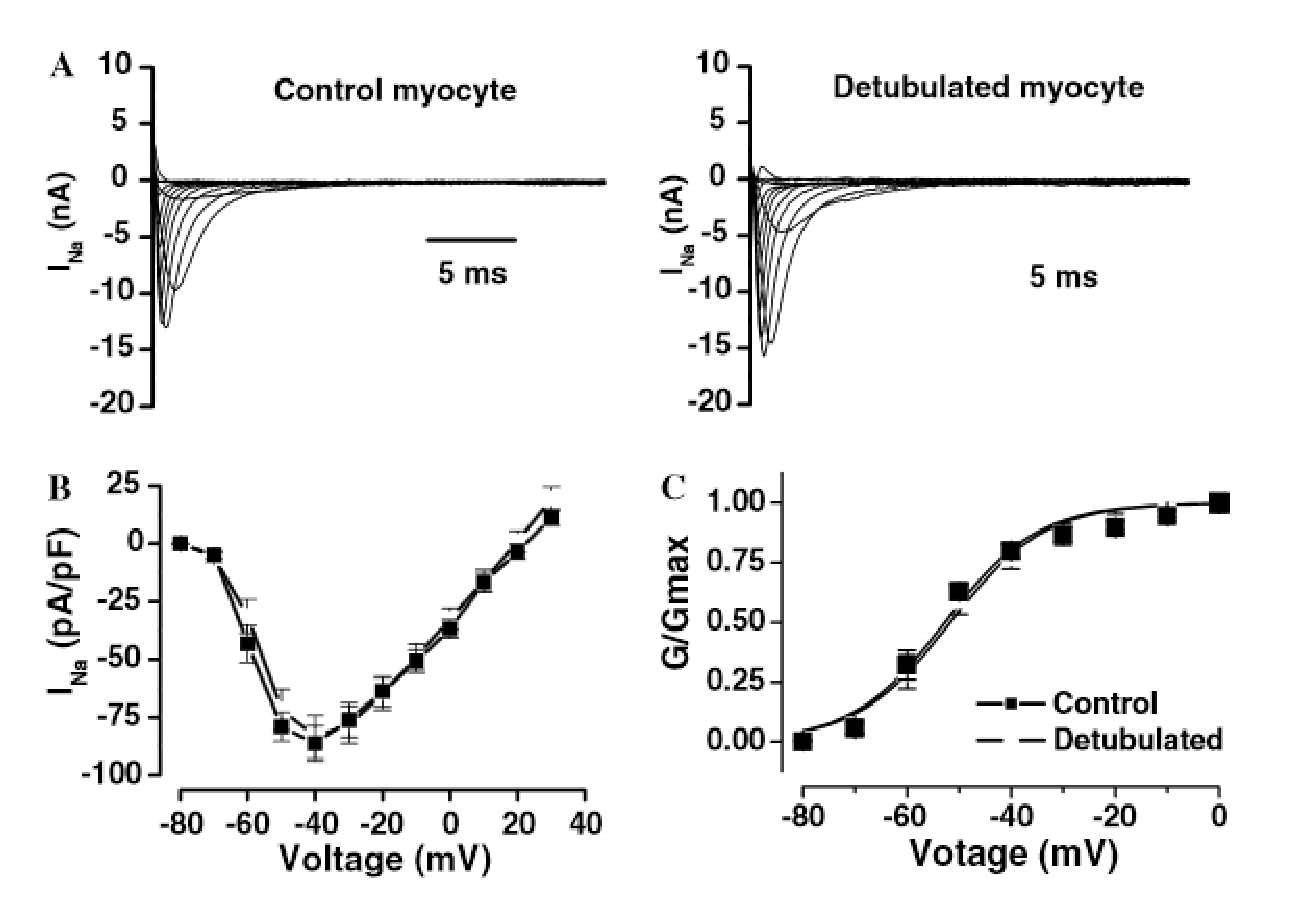
\includegraphics[height=5cm,
    angle=0]{./images/Ina_cardiac_brette2006.eps}}
  \caption{$I_\na$ in control and detubulated ventricular myocytes}
  \label{fig:Ina_cardiac_brette2006}
\end{figure}


To measure the $\Na$ currents, we need to block other currents:
\begin{enumerate}
  \item block $\K$ currents using internal and external application of TEA
  \item leak was subtracted electronically
\end{enumerate}


The activation curve is fitted with Boltzmann equation  (Sect.\ref{sec:Boltzmann-equation})
\begin{equation}
\label{eq:Boltzmann-equ}
a = \frac{1}{1+\exp\left( V_m - V_{1/2})/k \right)}
\end{equation}
with $a$ is activation variable, and $k$ the slope factor, $V_{1/2}$ is
the potential at the current of half-activated. 


\subsection{-- mutation SCN5A}

Mutation of this genes are associated with different arrhythmogenic syndromes:
including long QT syndrome (LQT3 and a peculiar polymorphic ventricular
tachycardia - Torsades de Pointes) \citep{wang1995, wang1995scn5a}, Brugada
syndrome \citep{weiss2002}, Lenegre disease (inherited cardiac conduction
defect).
\begin{itemize}
  \item  The mutation invariably disrupt the fast inactivation, and allow repeated
reopening during sustained depolarization, evoking a small, persistant $\Na$
current during the AP plateau \citep{Balser2001}, Fig.\ref{fig:I_Na_mutation}.

\begin{figure}[hbt]
  \centerline{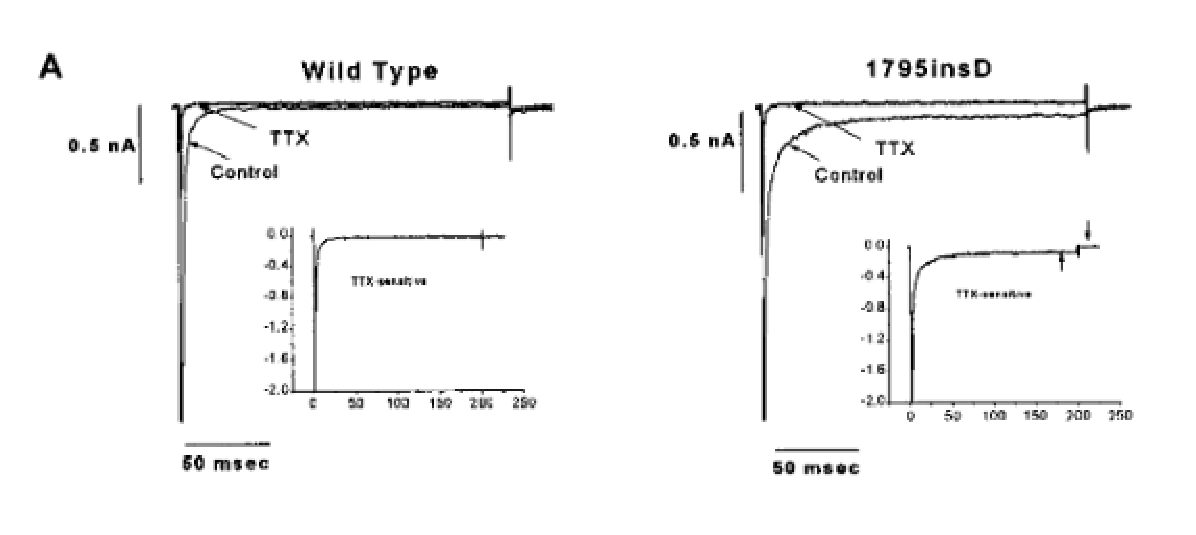
\includegraphics[height=5cm,
    angle=0]{./images/I_Na_mutation.eps}}
  \caption{Tetrodotoxin (TTX)-sensitive Na current: (A) Wild-type; (B) A
  mutation in the C-terminus}
  \label{fig:I_Na_mutation}
\end{figure}
  
\end{itemize}


\subsection{Coupled states Na channel}

Other studies suggested that 'coupled' model should be used. Indeed, the time
course of recovery during inactivation (i.e.
decay) exhibits two exponential components (one fast + one slow). Thus,
\citep{chiu1977} proposed 3-state inactivation model: one open and two closed
states (Sect.\ref{sec:Ina_Chiu1977}).

Summary: a $\Na$ channel can exist in one of the three hypothetical states:
resting, activated, and inactivated.
\section{Sodium transient current}
\label{sec:transient-sodium-current}

The conventional voltage-dependent TTX-sensitive sodium channels produce the
large, inward currents that underlie fast action potentials in neurons.

In certain cell types, the current may also present, with a smaller amount, at
rest which influence subthreshold electrical behavior, as suggested originally
by effects of tetrodotoxin (TTX) at subthreshold voltages (Hotson et al., 1979;
Llinas and Sugimori, 1980a).

\begin{enumerate}
  
  \item {\bf Nav1.1}:   Nav1.1 is predominantly expressed in the soma and
  proximal axon initial segment of fast-spiking GABAergic neurons
  
  
  \item {\bf Nav1.6}: Nav1.6 is found at the distal axon initial segment and
  nodes of Ranvier of both fast-spiking GABAergic and excitatory neurons.
  
 NOTE: an auxiliary voltage-gated sodium channel subunit, Nav$\beta$4, is also
 enriched in the axon initial segment of fast-spiking GABAergic neurons.
 
 The C-terminal tail of Nav$\beta$4 is thought to mediate resurgent sodium
 current (Sect.\ref{sec:resurgent-sodium-current}), an atypical current that
 occurs immediately following the action potential and is predicted to enhance
 excitability.
 
\end{enumerate}

\subsection{Resurrent sodium current (NaR)}
\label{sec:NaR-current}
\label{sec:resurgent-sodium-current}

Nav$\beta$4, an auxiliary subunit to sodium channel, is enriched in the AIS of
fast-spiking GABAergic neurons.The C-terminal of Nav$\beta$4 is thought to
mediate the {\bf resurgent sodium curent}. This is an atypically current that
occurs immediately following AP and is predicted to enhance excitability of the
cells (review: Patel, Cummins, 2015).

In Purkinje neurons, an unusual voltage- and time-dependent behavior of sodium
current in which repolarization from a voltage of +30 mV to voltages near -40 mV
elicits a transient current of several hundred picoamps. This 'resurgent' sodium
current, which is sensitive to TTX, is present in Purkinje neurons, but not
present in CA3 pyramidal neurons (Raman, Bean (1997)). On Purkinje neurons,
the peak is $\sim$ 120pA (at -30mV) with 50mM $\Na$ as charge carrier.

The channels underlying this resurgent sodium current also generate conventional
fastinactivating sodium current (Sect.\ref{sec:transient-sodium-current}).
This current has been found in 
\begin{enumerate}
  \item cerebellar Purkinje neuron (Raman, Bean (1997))

The peak is small, 3.5\% of the peak transient elicited by step from -90mV to
-30mV; but the resurrent current flows a longer time, i.e. a much slower decay
kinetics ($\tau = 30$ ms for resurrent current; vs. 1.5ms for transient current
at -30mV)
   
\end{enumerate}
but NOT in
\begin{enumerate}
  \item CA3 pyramidal neuron
\end{enumerate}

Nav$\beta$4 - the modulatory Na(+) channel subunit
(Sect.\ref{sec:Na-channel-beta-subunit}) - is thought to underlie resurgent
Na(+) current.
\begin{enumerate}
  \item  In cerebellum (Purkinje cells) and spinal cord, $\beta$4 is
  clustered/localized in AIS and nodes of Ranvier (like other $\beta$ subunits)

Here, Nav1.6 (Sect.\ref{sec:Nav1.6}) and $\beta$1 are also localized in the same
region.

  \item In striatal projection axons, however, $\beta$4 is diffusely distributed
  in axons  (Miyazaki, Nukina (2014))
 
 Neurons expressing $\beta$4 are mainly found in the striatum; with strongest
 $\beta$4 immunoreactivity was observed in GPe and SNr (i.e. in striatal
 projection neurons iSPN and dSPN).
 
 $\beta$4-deficient mice exhibit a reduction of INaR, disruption of
  repetitive firing and increased failure rates in medium spiny neurons (MSNs)
  in the striatum, suggesting that $\beta$4 serves as a physiological channel
  modulator in MSN.


\end{enumerate}

\section{Sodium persistent current}
\label{sec:persistent-sodium-current}

Some voltage-clamp experiments in many types of central neurons have shown the
existence of persistent or noninactivating sodium currents active at
subthreshold voltages (Stafstrom et al., 1985; French et al., 1990; Cepeda et
al., 1995). Such currents may play major roles in regulating repetitive firing,
amplifying dendritic depolarization, and producing afterdepolarizations and
plateau potentials (for review, see Taylor, 1993; Crill, 1996).

However, there is still little known about the channels that underlie these
currents.



 
\section{Na+ leak current}
\label{sec:Na-leak-channel}
\label{sec:leak-Na-channel}

Sodium leak current is considered contributing an important part to resting
membrane potential (Sect.\ref{sec:resting-membrane-potential}).

Ren (2011): reference (Atherton and Bevan, 2005; Eggermann et al., 2003; Jackson
et al., 2004; Jones, 1989; Khaliq and Bean, 2010; LeSauter et al., 2011; Pena
and Ramirez, 2004; Raman et al., 2000; Russo et al., 2007).


\subsection{Nalcn (non-selective)}
\label{sec:NALCN}
\label{sec:Nalcn}
%\label{sec:Nalcn-channel}

NALCN gene expresses a  Voltage-independent, non-selective cation Nalcn channel
(permeable to $\Na$, $\K$, and $\Ca$) that is widely expressed in the nervous
system. NALCN gene is at chromosome 13q33.1 (Gross, 2013).

\begin{itemize}
  \item Lee et al. (1999) first cloned in rat, with 4 subunits, each with 6TM/P
  (Sect.\ref{sec:6TM/P}).
  
  Rat and human NALCN shares 99\% identity.
  
  \item Northern blot analysis showed the dominant expressin is in 
  \begin{enumerate}
    
    \item  rat brain and  spinal cord horn neurons; and moderate expression in
    heart; weak expression in pancreas; not in  liver, muscle, kidney, or
    testis. (Lu et al., 2007)
  
    \item human brain (cerebellum, corpus callosum, cortex, brainstem, striatum,
    substantia nigra, putamen, pons, and spinal cord); not found in 
    nonneural tissues, including blood, liver, skeletal muscle, bone marrow, and
    adipose tissue (Koroglu et al., 2013); low expression in human muscle and
    fibroblast (Al-sayed et al., 2013)
  \end{enumerate}
  
\end{itemize}

Nalcn is responsible for the neuronal background Cs(+)- and TTX-resistant Na+
leak conductance and regulate neuronal excitability (Lu et al., 2007) -
Sect.\ref{sec:Na-current-TTX-resistant}, i.e. 
the Voltage-independent sodium current helps slightly depolarize
neurons. 

{\bf Activators}
\begin{itemize}
  
  \item  In mouse hippocampal and VTA neurons
  (Sect.\ref{sec:ventral-tegmented-area}), Nalcn is activated by substance P
  receptor - TACR1 (Sect.\ref{sec:substance-P-like-neuron}), rather than
  G-protein.
  
  substance P activate its receptor - TACR1 (162323) which is also a G
  protein-coupled receptor but occurs by means of a unique mechanism: it does
  not require G protein activation but is dependent on Src family kinases
  (Sect.\ref{sec:Src}).

  \item Activation of M3 muscarinic receptors by acetylcholine:  significantly
  increases NALCN currents,
  
  \item Activation of NK1 by Substance P:  significantly increases NALCN
  currents,
\end{itemize}

{\bf Inhibitor}
\begin{itemize}
  \item  Activation of CaSR ($\Ca$-sensing receptor) by extracellular calcium
  stops the flow of the currents (Sect.\ref{sec:GPCR-class-C})
\end{itemize}


Nalcn and Unc79 (Sect.\ref{sec:UNC79}) interacted directly with Unc80, but not
with each other. In addition, the channel also plays a major role in determining
the sensitivity to extracellular Ca2+ of neuronal excitability. However,
activation of Nalcn channel alone were insensitive to extracellular Ca(2+), and
Unc80 provided Ca2+ sensitivity. Unc79 appeared to contribute to Ca(2+)
sensitivity of Nalcn currents by interacting with Unc80 and stabilizing Unc80
protein level, based on the observation given below (review: Ren, 2011).
\begin{itemize}
  
  \item  Unc79 -/- hippocampal neurons showed normal Nalcn-dependent Na+ leak
  currents, but their leak currents were largely insensitive to changes in
  extracellular Ca(2+) concentration.
  
  \item Overexpress of Unc80 can bypass the requirement for Unc79, i.e. rescue
  extracellular $\Ca$-sensitivity.
\end{itemize}
\url{http://www.omim.org/entry/616884}


\subsection{-- UNC79}
\label{sec:UNC79}

UNC79 gene encode for the protein that (name as KIAA1409) functions as an
accessory subunit of the Nacln channel (Sect.\ref{sec:Nalcn}). It has 1,597
amino acids.

They are found  in adult and fetal brain, adult spinal cord, and in all specific
adult brain regions examined. Very weak expression was detected in pancreas,
with little to no expression detected in other adult and fetal tissues.

\subsection{-- UNC80}
\label{sec:UNC80}

UNC80 gene encodes a large protein (named as KIAA1843) necessary for the
stability and function of the Nalcn (Sect.\ref{sec:Nalcn}). The protein has
1,341 amino acids. 


\section{Pyramidal Nat}
\label{sec:Nat-Pyramial}

\subsection{CA1 hippocampal}
\label{sec:Nat-Pyramial-CA1-hippocampal}

Sah et al. (1988) 

\subsection{neocortical}
\label{sec:Nat-Pyramial-neocortical}

Huguenard, Hamill and Prince (1988) did whole-cell voltage-clamp on rat
neocortical neurons (both pyramidal and non-pyramidal neuron) from {\bf
sensorimotor area} isolated using their acute dissociation technique
(Sect.\ref{sec:technique-cell-dissociation}), measured at E16 (day 16) and at
P50 (postnatal, day 50) to quantify the developmental changes in kinetic
properties. 

NOTE: Pieces of cortex (600$\mum$) are incubated at 26$^\circ$C in {\bf
Bicarbonate-buffered saline} (in mM):
NaCl 130, KCl 5, $\ce{CaCl_2}$  1, $\ce{MgCl_2}$ 1, $\ce{NaHCO_3}$  26,
D-glucose 25 (i.e. dextrose 25), cysteine 0.01, 1.6 mg/ml papain (type IV,
Sigma), and HEPES 20 at pH 7.4.


RESULTS:
\begin{enumerate}
  
  \item {\bf conductance}: near 10 pS/$\mum^2$ (E16); and (when
  normalized to density value) increase 6- to 10-fold during first two week
  postnatal (P50). Yet, final conductance reached in pyramidal neurons was
  higher than in non-pyramidal neuron.
  
  The increase in conductance density can be explained by either
  (1) higher single-channel conductance (i.e. number of channel does not change
  much); (2) many more channels added. The recording data at single-channel
  level confirms the later option, i.e. more channels added.
  
  \item half-activation: $V_{1/2} = -32$ (mV) and slope $k = 6.5$ mV per e-fold
  change in activation; quite the same for both developmental and matured
  pyramidal neuron.
  
  
  \item \textcolor{red}{In E16 immature rat}:
  \begin{itemize}
  \item {\bf threshold for activation}: -55 mV
  
  \item {\bf I-V curve gives peak $I_\na$} (different voltage-clamp pulses):
  near -10 mV; with peak about 380 pA. (check Fig.2 in paper).
  
  Holding potential -100 mV; with +10 mV voltage step increment starting at -56
  mV for the duration 15 ms.

  \item {\bf f-V curve gives half-activation}: at $V_{1/2}=-29$ mV; slope
  $k=6.5$ (mV) per e-fold; peak conductance $\bar{g}_\na = 6.4$ nS based on
  Ohm's law 
  
  \begin{equation}
  I_{\text{peak},\na} = \bar{g}_\na \times (\Vm - E_{\rev,\na})
  \end{equation}
  
  \item can be fit using Hodgkin-Huxley formula: with activation is fit using
  monophasic exponential decay with time constant $\tau_h$.

  \item the time course of decay $\tau_h$ is independent from the values of
  $[\Na]_o$, i.e. it is indepenent of the current (Fig. 8 in the paper).
  
  \item {\bf maximal conductance}: 
  \end{itemize}
  
  \item \textcolor{red}{In P50 postnatal rat}:
  \begin{itemize}
    \item measurement was not easy at normal $[\Na]_o =145$ mM; so they also
    measured at reduce $[\Na]_o = 10 $mM
    
    \item {\bf maximal conductance}: 131 nS (normal $[\Na]_o$) and 7 nS (at
    reduced $[\Na]_o$)
    
    \item the decay has 2 components: 
    
\begin{equation}
I_\na = I_{\na,f} + I_{\na,s}
\end{equation}


  \end{itemize}
  
\end{enumerate}

\section{Non-pyramidal neocortical neuron Nat}


A similar work done by Huguenard, Hamill and Prince (1988) which compared
non-pyramidal neocortical neuron vs. pyramidal neuron in sensorimotor
area (see also Sect.\ref{sec:Nat-Pyramial-neocortical}).
\begin{enumerate}
  \item no kinetics difference, i.e. we can use kinetics from Pyramial neuron
  for non-pyramidal neuron
  
  The difference in AP is thus explained by the difference in current density
  (see in Sect.\ref{sec:Nat-Pyramial-neocortical}), i.e. change in the number of
  channels per unit membrane area - which underlies the increased rate of rise of AP.
  
  
  \item 
\end{enumerate}

\section{Neostriatal neuron}

\subsection{Ogata, Tatebayashi (1990) - rat}

NOTE - Incubation (1 hour, with continuously bubbled with 100\% O2): Pieces of
cortex (600$\mum$) are incubated at 36$^\circ$C in {\bf Bicarbonate-buffered saline} (in mM):
NaCl 120, KCl 5, $\ce{CaCl_2}$  1.8, $\ce{MgCl_2}$ 1, 
piperazine-N,N'-bis[2-ethanesulfonic acid]Na (PIPES-Na)
%$\ce{NaHCO_3}$  26,
D-glucose 25, trypsin 0.5\%.
%, 1.6 mg/ml papain (type IV, Sigma), and HEPES 20 at pH 7.4.

After that, the slices were gently agitated with a fire-polished pasteur pipette
(inner tip diameter, 100 $\mum$).

Electrical recording was based on  whole-cell variation of
the patch-clamp technique (Hamill et al. 1981) -
Sect.\ref{sec:patch-clamp-whole-cell}.
\begin{itemize}
  \item suction pipette: resistance 1.2-2 M$\Omega$
  
  \item membrane current passing through the pipetter was recorded using
  current-to-voltage converter designed by M. Yoshii (Narahashi et al., 1987)
  
  \item the command pulse is adjusted to compensate the effect caused by total
  resistance - the decay of capacitive current was speed up for compensation
  
  The decay phase of the capacitive transient was
well described by a single exponential function before and after series
resistance compensation.
  % Sect.\ref{sec:bridge-balance}
  
  \item Capacitative and leakage currents were subtracted digitally by the P-P4
  procedure (Bezanilla and Anlastrong 1977) - Sect.\ref{sec:leak-current-subtraction}

  \item The liquid junction potential between internal and external solutions
  were about -13 mV (and the data shown is adjusted after this)
  
  \item the solution for pipette is discussed in Sect.\ref{sec:electrode-electrolyte-solution}
\end{itemize}


\textcolor{red}{RESULTS}
\begin{enumerate}
  
  \item {\bf activation curve}:  activated at -60 mV; peak current: at -20 mV
  (of value -2 nA); Vrev = +60 mV (from Nernst equation) (or +54 mV from the I/V
  curve); half activation:$V_{1/2} = -25$ (mV) and slope k = 10 (mV).
  (Fig. 3A).
  
  
  time constant (curve has bell-shape configuration): increase value (reaching
  peak at -60 mV) and then decrease (Fig. 5).
  
  \begin{itemize}
    \item at -100 mV: 0.3162 (ms)
    \item at -90 mV: 0.3162 (ms)
    \item at -80 mV: 0.3512 (ms)
    \item at -70 mV: 0.4474 (ms)
    \item at -60 mV: 0.5566 (ms)
    \item at -50 mV: 0.3548 (ms)
    \item at -40 mV: 0.2399 (ms)
    \item (at -30mV) 0.16$\pm$0.02 (ms)
    \item at -20 mV: 0.1047 (ms)
    \item at -10 mV: 0.0871 (ms)
    \item at 0 mV: 0.0851 (ms)
    \item at +10 mV: 0.0813 (ms)
    \item at +20 mV: 0.0832 (ms)
    \item at +30 mV: 0.0832 (ms)
    \item at +40 mV: 0.0832 (ms)
    \item at +50 mV: 0.0832 (ms)
  \end{itemize}  
  
  \item {\bf inactivation curve}: $V_{1/2} = -62$ (mV); slope k = 6 (mV)
  
  time constant (also bell-shape configuration): increase slowly (reach peak
  value at -60 mV) and then decrease. 
  
  They found that the inactivation was a two-order process; particularly at
  relatively negative activation levels. So, two components of inactivation were
  found; and below are the values for the fast component
\begin{itemize}
    \item at -100 mV:5.9196 (ms),  
    \item at -90 mV: 5.9196 (ms)
    \item at -80 mV: 5.9197 (ms)
    \item at -70 mV: 6.9103 (ms)
    \item at -60 mV: 8.2985 (ms)
    \item at -50 mV: 3.9111 (ms)
    \item at -40 mV: 1.4907 (ms)
    \item (at -30mV) 0.6596 (ms)
    \item at -20 mV: 0.5101 (ms)
    \item at -10 mV: 0.4268 (ms)
    \item at 0 mV: 0.3673 (ms)
    \item at +10 mV: 0.3370 (ms)
    \item at +20 mV: 0.3204 (ms)
    \item at +30 mV: 0.3177 (ms)
    \item at +40 mV: 0.3151 (ms)
    \item at +50 mV: 0.3142 (ms)
\end{itemize}   
NOTE: The slow component may arises from a subset of Na channels with delayed
opening or multiple reopening during a step depolarization. 
Another explanation is that the two exponential components arised from two
subsets of Na channels with different mean channel-open times.
The result supported the multiple reopening or delayed opening with a single
inactivated state.
  
\end{enumerate}

\subsection{Pisani, Calabresi (1995) - rat}
\label{sec:drug-felbamate-FBM}
\label{sec:felbamate}
\label{sec:Nat-striatal-neuron-Pisani-calabresi-1995}
\label{sec:FBM}

\textcolor{red}{RESULTS}
\begin{enumerate}
   \item {\bf activation curve}:  
%   activated at -60 mV;  
%   peak current: at -20 mV; Vrev = +60 mV (from Nernst equation) (or +54 mV from
%   the I/V curve); half activation:$V_{1/2} = -25$ (mV) and slope k = 10 (mV).
%   (Fig. 3A)
%   
Tested with holding -70 mV, and then depolarize step pulse +10mV, until to -20
mV.
    
%   time constant (curve has bell-shape configuration): increase value (reaching
%   peak at -60 mV) and then decrease (Fig. 5).
%   
%   \begin{itemize}
%     \item (at -30mV) 0.16$\pm$0.02 (ms)
%   \end{itemize}  
 
  from holding -70 mV to -20mV: it induces INa with peak 1200 (pA), i.e.
  1.2 nA, total current. 
   
  \item {\bf inactivation curve}: $V_{1/2} = -50$ (mV); slope k = 7.29 (mV)
  
  Tested with holding -70 mV, and then hyperpolarize step pulse -10mV, until to
  -110 mV.
  
%   time constant (also bell-shape configuration): increase slowly (reach peak
%   value at -60 mV) and then decrease.
  
\end{enumerate}


Anticonvulsant drug {\bf felbamate} (FBM) is tested its
effect on striatal neurons.
\begin{itemize}
  
  \item (2-phenyl-1,3-propanediol-dicarbamate) = FBM

NOTE: FBM shows its role as an antileptic drug, e.g. an neuroprotectant
agent:  effective in the treatment of partial onset seizures
(Sect.\ref{sec:seizure-drug}) and in the Lennox-Gastaut syndrome.
  
  \item at theurapatically relevant concentration (30 - 300 $\muM$)
  
  \item a dose-related effect on reduction of $\Na$ current (tested with 10-100
  $\muM$) with IC50 is 28 $\muM$.
  
  FBM shifts inactivation curve to the more negative value by 10.4mV (without
  clear modification of the slope).
  
  \item at 1.2mM $\Mg$ control condition: FBM does not affect corticalstriatal
  glutamatergic transmission, based on the fact that EPSP (intracellular
  recording) and field potential - Sect.\ref{sec:field-potential} (extracellular
  recording) not change.
  
  \item without $\Mg$ block: dose-related effect on NMDA-current (postsynaptic
  level) on the amplitude of field potential and EPSP.
  
\end{itemize}


\textcolor{red}{Protocols}:
\begin{enumerate}
  \item adult male Winstar rat (200-250 g)
  
  \item coronal slice (450$\mum$ thickness), incubated in 
  HEPES-buffered Hank's balanced salt solution (HBSS), bubbled with 100\% 02 and
  warmed at 34$^\circ$C; and enzymatic treatment
  (Sect.\ref{sec:enzymatic-treatment-technique-dissociate-cells}).
  
{\bf Incubation} in solution containing (in mM): sodium chloride (NaCl) 126,
potassium chloride (KCl) 2.5, monosodium acid phosphate (NaH2PO4) 1.2, magnesium
chloride (MgCl2) 1.2; calcium chloride (CaCl) 2.4, glucose 10 and sodium
carbonate (NaHCO3) 26; the solution was gassed with a mixture of 02 (95\%) and
CO2, (5\%).

In some experiments MgCl2 was omitted from the solution.
  
   \item extracellular electrode: 2 M NaCl; 
   
   \item intracellular recording electrodes were filled with either 2 M KCl or 
   2M K-acetate (30-60 M$\Omega$).
   
   \item for synaptic stimulation, bipolar electrodes were used.
   
 These were placed in the cortex, close to the recording electrode, or in the
 white matter between the cortex and the striatum.
  
\end{enumerate}

\subsection{Siep, Kohling (2001) - hamster}
\label{sec:Nat-striatal-Siep-Kohling-2001}
\label{sec:dystonic-mutant-hamster}
\label{sec:paroxysmal-dystonia-hamster-model}


Dystonic mutant \dtsz hamsters are a model for paroxysmal dystonia.

The effect of lamotrigine was tested on healthy vs. \dtsz hamster on 
on (a) current/voltage relationship, (b) kinetics, and (c) steady-state inactivation
and activation of INa current.


\textcolor{red}{RESULTS}: Study INa in healthy vs. \dtsz hamster with whole-cell
clamp recording. Holding potential -80 mV. Tight-seal whole-cell
recordings were obtained using the method of Hamill et al. (1981) with seal
resistances > 1 G$\Omega$.
 
\begin{enumerate}
  
  \item estimated cell capacitance: 5.3 $\pm$ 0.6 (pF)
  
  Assuming value of $\Csc = 1 \muF/\cm^2$; sodium conductance and current
  density was very high (> 280 pS/cm$^2$; or > 2000 pA/pF).
  
  \item {\bf activation curve}:  (threshold for activation) activated at -65 to
  -55 mV; %peak current: at -20 mV; Vrev = +60 mV (from Nernst equation) (or
  % +54 mV from the I/V curve); 
  half activation:$V_{1/2} = -31.2 \pm 0.5$ (mV) and 
  %slope k = 10 (mV).
  %(Fig. 3A)

  As native INa currents was found quite large (> 10 nA or > 10,000 pA), the
  current had to be reduced using the procedure described by Huguenard et al.
  (1988) and Reckziegel et al. (1998). Under these conditions, maximal
  INa current amplitudes was 1.2 nA peak at -16.6 mV. 

   
   time constant with value
   \begin{itemize}
     \item 0.25 $\pm$ 0.08 (ms) at -20 mV in healthy; and 0.19 (ms) in \dtsz 
   \end{itemize}  
%   time constant (curve has bell-shape configuration): increase value (reaching
%   peak at -60 mV) and then decrease (Fig. 5).
%   
%   \begin{itemize}
%     \item (at -30mV) 0.16$\pm$0.02 (ms)
%   \end{itemize}  
%   
   \item {\bf inactivation curve}: $V_{1/2} = -75$ (mV); slope k = 8.1 (mV)
	
	Under CTRL, at a resting membrane potential of approximately -80 mV, only
	about 50\%  of the channels are available for action-potential generation. 
	
   time constant
   \begin{itemize}
     \item 1.15 $\pm$ 0.08 (ms) at -20 mV in healthy; and 0.96 (ms) in \dtsz
     
     
   \end{itemize}
%   time constant (also bell-shape configuration): increase slowly (reach peak
%   value at -60 mV) and then decrease.
  
\end{enumerate}




\textcolor{red}{Protocols}: (based on Pisani, Calabresi (1995))
\begin{enumerate}
  \item postnatal P21 and P30 hamster (200-250 g)
  
  \item coronal slice (500$\mum$ thickness), incubated in 
  HEPES-buffered Hank's balanced salt solution (HBSS), bubbled with 100\% 02 and
  warmed at 32$^\circ$C; and enzymatic treatment with 1.0 mg/ml trypsin
  (Sect.\ref{sec:enzymatic-treatment-technique-dissociate-cells}).
  
{\bf Incubation} in solution containing (in mM): sodium chloride (NaCl)
\textcolor{red}{120}, potassium chloride (KCl) \textcolor{red}{5}, magnesium
chloride (MgCl2) \textcolor{red}{1}; calcium chloride (CaCl2)
\textcolor{red}{1}, PIPES 20; glucose \textcolor{red}{25}; with pH 7.0; the
solution was gassed with a mixture of 02 (95\%) and CO2, (5\%).

%no: , monosodium acid phosphate (NaH2PO4) 1.2,  and sodium carbonate
% (NaHCO3) 26
  
   \item extracellular electrode: 2 M NaCl; 
   
   \item intracellular recording electrodes were filled with either 2 M KCl or 
   2M K-acetate (30-60 M$\Omega$).
   
   \item for synaptic stimulation, bipolar electrodes were used.
   
 These were placed in the cortex, close to the recording electrode, or in the
 white matter between the cortex and the striatum.
  
\end{enumerate}
